\subsection{Ôn tập chương VII}
\Opensolutionfile{ans}[ans/ans-1K7-27-OTC]

\begin{ex}%[Đỗ Minh Phúc]%[1K7BL-1]%
	Trong không gian cho đường thẳng $a$ và điểm $ M $. Có bao nhiêu đường thẳng qua $ M $, cắt $a$ và vuông góc với $a $?
	\choice
	{$1$}
	{$2$}
	{Vô số}
	{\True Có $1$ hoặc vô số}
	\loigiai{
		Có $1$ nếu $M$ không thuộc $a$ và có vô số nếu  $ M $ thuộc $ a $.
	}
\end{ex}

\begin{ex}%[Đỗ Minh Phúc]%[1K7YL-1]%
	Trong các mệnh đề sau, mệnh đề nào đúng?
	\choice
	{Trong không gian, nếu hai đường thẳng phân biệt cùng vuông góc với một đường thẳng thứ ba thì hai đường thẳng đó song song với nhau}
	{Trong không gian, nếu một đường thẳng bất kì vuông góc với một trong hai đường thẳng song song thì đường thẳng đó song song với đường thẳng còn lại}
	{Trong không gian, nếu hai đường thẳng phân biệt cùng vuông góc với một đường thẳng thứ ba thì hai đường thẳng đó vuông góc với nhau}
	{\True Trong không gian, hai đường thẳng vuông góc với nhau thì chéo nhau hoặc cắt nhau}
	\loigiai{Mệnh đề đúng là: \lq \lq Trong không gian, hai đường thẳng vuông góc với nhau thì chéo nhau hoặc cắt nhau\rq \rq.
		
	}
\end{ex}

% \begin{ex}%[Đỗ Minh Phúc]%%
	%	Cho hình chóp đều, chọn mệnh đề \textbf{sai} trong các mệnh đề sau
	%	\choice 
	%	{ Chân đường cao của hình chóp đều trùng với tâm của đa giác đáy đó} 
	%	{ \True Tất cả những cạnh của hình chóp đều bằng nhau} 
	%	{ Đáy của hình chóp đều là miền đa giác đều} 
	%	{ Các mặt bên của hình chóp đều là những tam giác cân}
	%	\loigiai{
		%		Hình chóp đều có thể có cạnh bên và cạnh đáy không bằng nhau nên phương án \lq\lq  Tất cả những cạnh của hình chóp đều bằng nhau\rq\rq\, là sai.}
	%\end{ex}   
	\begin{ex}%[Đỗ Minh Phúc]%[1K7YL-1]%
		Trong các mệnh đề sau đây, mệnh đề nào đúng?
		\choice 
		{ Hai đường thẳng phân biệt cùng vuông góc với một đường thẳng thì song song với nhau} 
		{ \True Hai mặt phẳng phân biệt cùng vuông góc với một đường thẳng thì song song với nhau} 
		{ Hai mặt phẳng phân biệt cùng vuông góc với một mặt phẳng thì song song với nhau} 
		{ Hai đường thẳng phân biệt cùng song song với một mặt phẳng thì song song với nhau}
		\loigiai{
			\begin{itemize}
				\item Hai đường thẳng phân biệt cùng vuông góc với một đường thẳng thì song song với nhau. sai vì có thể hai đường thẳng chéo nhau.
				\item Hai mặt phẳng phân biệt cùng vuông góc với một mặt phẳng thì song song với nhau. sai vì hai mặt phẳng có thể cắt nhau theo một giao tuyến vuông góc với mặt phẳng đã cho.
				\item Hai đường thẳng phân biệt cùng song song với một mặt phẳng thì song song với nhau. sai vì hai đường thẳng có thể chéo nhau hoặc cắt nhau.
			\end{itemize}
		} 
	\end{ex}
	
	\begin{ex}%[Đỗ Minh Phúc]%[1K7YL-3]%
		Cho hình lập phương $ ABCD.A'B'C'D'$. Đường thẳng nào sau đây vuông góc với đường thẳng $A'B?$
		\choice
		{$CC'$}
		{$AC$}
		{$CD$}
		{\True $DC'$}
		\loigiai{
			\immini{Ta có $ABA'B'$ là hình vuông nên $ A'B\perp AB'$\\
				mà $ AB' \parallel C'D$\\
				nên $ A'B\perp C'D.$}
			{\begin{tikzpicture}[font=\footnotesize, line join=round, line cap=round, >=stealth]
					\def\r{2.5}
					\path
					(0,0) coordinate (A)
					++(0:\r) coordinate (B)
					++(30:0.7*\r) coordinate (C)
					($(A)+(C)-(B)$) coordinate (D)
					\foreach \x in {A,B,C,D}
					{($(\x) + (90:\r)$) coordinate (\x')}
					;
					\draw [dashed]
					(A)--(D)--(C) (C')--(D)--(D')
					;
					\draw
					(A)--(A')--(D')--(C')--(C)--(B)--(A)
					(B)--(A')--(B')--(B) (A)--(B')--(C')
					;
					\foreach \x/\y in {A/-150,B/-30,C/0,D/160,A'/180,B'/-30,C'/0,D'/150}
					\draw[fill = black] (\x) circle (.03cm) + (\y:.3cm) node {$\x$};
			\end{tikzpicture}}
		}
	\end{ex}
	
	\begin{ex}%[Đỗ Minh Phúc]%[1K7BO-2]%
		\immini{Cho hình chóp $S.ABC$ có đáy là tam giác vuông tại $A$ và cạnh bên $SA$ vuông góc với mặt phẳng đáy $(ABC)$ (minh họa hình bên). Khẳng định nào sau đây \textbf{sai}?
			\choice
			{$(SAB)\perp(SAC)$}
			{\True $(ABC)\perp(SBC)$}
			{$(SAC)\perp(ABC)$}
			{$(SAB)\perp(ABC)$}
		}
		{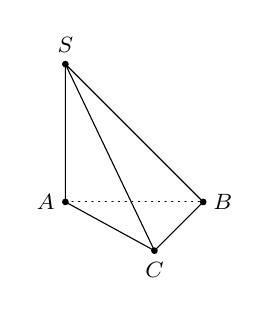
\begin{tikzpicture}[font=\footnotesize, line join=round, line cap=round, >=stealth]%Hinhchop
				\def\a{1.75}
				\def\b{0.5*\a}
				\path(0,0)coordinate(A)++(\a,0)coordinate(B)++(-135:\b)coordinate(C)(A)++(90:\a)coordinate(S);
				\draw[dotted](A)--(B);
				\draw(S)--(C)--(B)--cycle (S)--(A)--(C);
				\foreach \d/\g in{A/180,C/-90,B/0,S/90}
				\draw[fill=black](\d) circle(1pt)node[shift={(\g:0.25)}]{$\d$};
			\end{tikzpicture}		
		}
		\loigiai{
			\begin{itemize}
				\item $(SAB)\perp (SAC)$ đúng do $AB\perp (SAC),\,AB\subset (ABC)$.
				\item $(ABC)\perp (SBC)$ sai do hình chiếu vuông góc của $S$ lên $(ABC)$ là $A\notin BC$.
				\item $(SAC)\perp (ABC)$ đúng do $SA\perp (ABC),\,SA\subset (SAC)$.
				\item $(SAB)\perp (ABC)$ đúng do $SA\perp (ABC),\,SA\subset(SAB)$
			\end{itemize}
		}
	\end{ex}
	
	%\begin{ex}%[Đỗ Minh Phúc]%
	%	Góc giữa hai đường thẳng bất kỳ trong không gian là góc nào trong các góc dưới đây.
	%	\choice
	%	{Góc giữa hai đường thẳng cắt nhau và không song song với chúng}
	%	{Góc giữa hai đường thẳng lần lượt vuông góc với chúng}
	%	{\True Góc giữa hai đường thẳng cùng đi qua 1 điểm và lần lượt song song với chúng}
	%	{Góc giữa hai đường thẳng cắt nhau và lần lượt vuông góc với chúng}
	%	\loigiai{
		%		Dựa vào định nghĩa góc giữa hai đường thẳng.}
	%\end{ex}
	
	\begin{ex}%[Đỗ Minh Phúc]%[1K7BL-1]% 
		Mệnh đề nào sau đây là đúng?
		\choice
		{Góc giữa hai đường thẳng $a$ và $b$ bằng góc giữa hai đường thẳng $a$ và $c$ thì $b$ song song với $c$}
		{Góc giữa hai đường thẳng bằng góc giữa hai véc-tơ chỉ phương của hai đường thẳng đó}
		{Góc giữa hai đường thẳng là góc nhọn}
		{\True Góc giữa hai đường thẳng $a$ và $b$ bằng góc giữa hai đường thẳng $a$ và $c$ khi $b$ song song hoặc trùng với $c$}
		\loigiai{
			\begin{itemize}
				\item  Góc giữa hai đường thẳng $a$ và $b$ bằng góc giữa hai đường thẳng $a$ và $c$ thì hoặc $b \parallel c$ là phát biểu sai vì $b$ có thể trùng với $c$
				\item Góc giữa hai đường thẳng bằng góc giữa hai véc-tơ chỉ phương của hai đường thẳng đó là phát biểu sai vì góc giữa hai đường thẳng thuộc $\left[0^{\circ}; 90^{\circ}\right]$ còn góc giữa hai véc-tơ thuộc $\left[0^{\circ}; 180^{\circ} \right]$
				\item  Góc giữa hai đường thẳng là góc nhọn là phát biểu sai vì góc giữa hai đường thẳng có thể bằng $90^{\circ}$.
			\end{itemize}	
		}
	\end{ex}
	
	\begin{ex}%[Đỗ Minh Phúc]%[1K7BM-1]%
		Mệnh đề nào sau đây \textbf{sai}?
		\choice 
		{ Hai mặt phẳng phân biệt cùng vuông góc với một đường thẳng thì song song} 
		{\True Hai đường thẳng phân biệt cùng vuông góc với một đường thẳng thứ ba thì song song} 
		{ Một đường thẳng và một mặt phẳng cùng vuông góc với một đường thẳng thì song song nhau} 
		{ Hai đường thẳng phân biệt cùng vuông góc với một mặt phẳng thì song song	}
		\loigiai{
			Hai đường thẳng phân biệt cùng vuông góc với một đường thẳng thứ ba thì song song sai vì, Hai đường thẳng phân biệt cùng vuông góc với một đường thẳng thì có thể cắt nhau, chéo nhau.}
	\end{ex}
	
	%\begin{ex}%[Đỗ Minh Phúc]%
	%	Khẳng định nào sau đây \textbf{sai}?
	%	\choice 
	%	{ Nếu đường thẳng $d$ vuông góc với hai đường thẳng cắt nhau nằm trong $( \alpha )$ thì $d$ vuông góc với bất kì đường thẳng nào nằm trong $( \alpha )$} 
	%	{ Nếu đường thẳng $d\perp ( \alpha )$ thì $d$ vuông góc với hai đường thẳng trong $( \alpha )$} 
	%	{\True Nếu đường thẳng $d$ vuông góc với hai đường thẳng nằm trong $( \alpha )$ thì $d\perp ( \alpha )$} 
	%	{ Nếu $d\perp ( \alpha )$ và đường thẳng $a\parallel ( \alpha )$ thì $d\perp a$	}
	%	\loigiai{
		%		Nếu đường thẳng $d$ vuông góc với hai đường thẳng cắt nhau nằm trong $( \alpha )$ thì $d\perp ( \alpha )$.}
	%\end{ex}
	\begin{ex}%[Đỗ Minh Phúc]%[1K7BM-1]%
		Trong không gian cho đường thẳng $\Delta$ không nằm trong mp $( P )$, đường thẳng $\Delta$ được gọi là vuông góc với mp $( P )$ nếu
		\choice 
		{ vuông góc với hai đường thẳng phân biệt nằm trong mp $( P )$} 
		{ vuông góc với đường thẳng $a$ mà $a$ song song với mp $( P )$ } 
		{ vuông góc với đường thẳng $a$ nằm trong mp $( P )$} 
		{\True vuông góc với mọi đường thẳng nằm trong mp $( P )$}
		\loigiai{
			Đường thẳng $\Delta$ được gọi là vuông góc với mặt phẳng $( P )$ nếu $\Delta$ vuông góc với mọi đường thẳng trong mặt phẳng $( P )$.
		}
	\end{ex}
	%\begin{ex}%[Đỗ Minh Phúc]%
	%	Khẳng định nào sau đây \textbf{sai}?
	%	\choice 
	%	{ Nếu đường thẳng $d\perp ( \alpha )$ thì $d$ vuông góc với hai đường thẳng trong $( \alpha )$} 
	%	{\True  Nếu đường thẳng $d$ vuông góc với hai đường thẳng nằm trong $( \alpha )$ thì $d\perp ( \alpha )$} 
	%	{ Nếu đường thẳng $d$ vuông góc với hai đường thẳng cắt nhau nằm trong $( \alpha )$ thì $d$ vuông góc với bất kì đường thẳng nào nằm trong $( \alpha )$} 
	%	{ Nếu $d\bot ( \alpha )$ và đường thẳng $a//( \alpha )$ thì $d\bot a$}
	%	\loigiai{
		%		Theo định lý về điều kiện để đường thẳng vuông góc với mặt phẳng, để đường thẳng $d\perp ( \alpha )$ thì $d$vuông góc với hai đường thẳng cắt nhau nằm trong $( \alpha )$.
		%	}
	%\end{ex}
	\begin{ex}%[Đỗ Minh Phúc]%[1K7BM-1]%
		Cho hai đường thẳng $a$, $b$ và mp$(P)$. Chỉ ra mệnh đề đúng trong các mệnh đề sau
		\choice 
		{ Nếu $a\parallel ( P )$ và $b\perp a$ thì $b\parallel ( P )$}
		{\True Nếu $a\parallel ( P )$ và $b\perp ( P )$ thì $a\perp b$} 
		{ Nếu $a\parallel ( P )$ và $b\perp a$ thì $b\perp ( P )$}
		{ Nếu $a\perp ( P )$ và $b\perp a$ thì $b\parallel ( P )$}
		\loigiai{
			\begin{itemize}
				\item Nếu $a\parallel ( P )$ và $b\perp a$ thì $b\parallel ( P )$ là sai vì $b$ có thể vuông góc với $a$.
				\item Nếu $a\parallel ( P )$ và $b\perp ( P )$ thì $a\perp b$ là đúng bởi $a//( P )\Rightarrow \exists a'\subset ( P )$ sao cho $a//a',\,b\bot ( P )\Rightarrow b\bot a'$. Khi đó $a\bot b$.
				\item Nếu $a\parallel ( P )$ và $b\perp a$ thì $b\perp ( P )$ là sai vì $b$ có thể nằm trong $( P )$
				\item Nếu $a\perp ( P )$ và $b\perp a$ thì $b\parallel ( P )$ là sai vì $b$ có thể nằm trong $( P )$
			\end{itemize}
		}
	\end{ex}
	\begin{ex}%[Đỗ Minh Phúc]%[1K7BO-1]%
		Trong các mệnh đề sau đây, mệnh đề nào là đúng?
		\choice 
		{ Nếu hai mặt phẳng vuông góc với nhau thì mọi đường thẳng thuộc mặt phẳng này sẽ vuông góc với mặt phẳng kia} 
		{ Hai mặt phẳng phân biệt cùng vuông góc với một mặt phẳng thứ ba thì song song với nhau} 
		{ Với mỗi điểm $A\in ( \alpha )$ và mỗi điểm $B\in ( \beta )$ thì ta có đường thẳng $AB$ vuông góc với giao tuyến $d$ của $( \alpha )$ và $( \beta )$ } 
		{\True  Nếu hai mặt phẳng $( \alpha )$ và $( \beta )$ đều vuông góc với mặt phẳng $( \gamma )$ thì giao tuyến $d$ của $( \alpha )$ và $( \beta )$ nếu có sẽ vuông góc với $( \gamma )$}
		\loigiai{
			\begin{itemize}
				\item Nếu hai mặt phẳng vuông góc với nhau thì mọi đường thẳng thuộc mặt phẳng này sẽ vuông góc với mặt phẳng kia là sai vì nếu hai mặt phẳng vuông góc với nhau thì mọi đường thẳng thuộc mặt phẳng này vuông góc với giao tuyến sẽ vuông góc với mặt phẳng kia.
				\item Hai mặt phẳng phân biệt cùng vuông góc với một mặt phẳng thứ ba thì song song với nhau là sai vì còn trường hợp hai mặt phẳng cắt nhau.
				\item Với mỗi điểm $A\in ( \alpha )$ và mỗi điểm $B\in ( \beta )$ thì ta có đường thẳng $AB$ vuông góc với giao tuyến $d$ của $( \alpha )$ và $( \beta )$ là sai.
		\end{itemize}}
	\end{ex}
	\begin{ex}%[Đỗ Minh Phúc]%[1K7BM-1]%
		Chỉ ra mệnh đề \textbf{sai} trong các mệnh đề sau
		\choice 
		{\True  Cho hai đường thẳng vuông góc với nhau, mặt phẳng nào vuông góc với đường thẳng này thì cũng vuông góc với đường thẳng kia} 
		{ Hai đường thẳng phân biệt cùng vuông góc với một mp thì song song với nhau} 
		{ Cho hai mp song song, đường thẳng nào vuông góc với mặt mp này thì cũng vuông góc với mp kia} 
		{ Cho hai đường thẳng song song, mặt phẳng nào vuông góc với đường thẳng này thì cũng vuông góc với đường thẳng kia}
		\loigiai{
			Vì qua một đường thẳng dựng được vô số mặt phẳng.}
	\end{ex}
	
	\begin{ex}%[Đỗ Minh Phúc]%[1K7BM-1]% 
		Cho hai đường thẳng phân biệt $a$, $b$ và mặt phẳng $( P )$, trong đó $a\perp ( P )$. Chọn mệnh đề \textbf{sai}.
		\choice 
		{ \True Nếu $b\parallel a$ thì $b\parallel ( P )$}
		{ Nếu $b\parallel a$ thì $b\perp ( P )$} 
		{ Nếu $b\perp ( P )$ thì $b\parallel a$}
		{ Nếu $b\parallel ( P )$ thì $b\perp a$}
		\loigiai{
			Nếu $a\perp ( P )$ và $b\parallel a$ thì $ b\perp  ( P )$}
	\end{ex} 
	\begin{ex}%[Đỗ Minh Phúc]%[1K7BM-1]%
		Chọn mệnh đề đúng trong các mệnh đề sau đây
		\choice 
		{ Qua một điểm có duy nhất một mặt phẳng vuông góc với một mặt phẳng cho trước} 
		{ \True Cho hai đường thẳng chéo nhau $a$ và $b$ đồng thời $a\perp b$. Luôn có mặt phẳng $( \alpha )$ chứa $a$ và $( \alpha )\perp b$} 
		{ Cho hai đường thẳng $a$ và $b$ vuông góc với nhau. Nếu mặt phẳng $( \alpha )$chứa $a$ và mặt phẳng $( \beta )$ chứa $b$ thì $( \alpha )\perp ( \beta )$} 
		{ Qua một đường thẳng có duy nhất một mặt phẳng vuông góc với một đường thẳng khác	}
		\loigiai{
			\begin{itemize}
				\item Cho hai đường thẳng chéo nhau $a$ và $b$ đồng thời $a\perp b$. Luôn có mặt phẳng $( \alpha )$ chứa $a$ và $( \alpha )\perp b$. Đúng.
				\item 	Có vô số mặt phẳng đi qua một điểm và vuông góc với một mặt phẳng cho trước. Do đó, Qua một điểm có duy nhất một mặt phẳng vuông góc với một mặt phẳng cho trước là sai.
				\item 	Nếu hai đường thẳng $a$ và $b$ vuông góc với nhau và cắt nhau thì mặt phẳng chứa cả $a$ và $b$ không thể vuông góc với $b$. Do đó, Cho hai đường thẳng $a$ và $b$ vuông góc với nhau. Nếu mặt phẳng $( \alpha )$chứa $a$ và mặt phẳng $( \beta )$ chứa $b$ thì $( \alpha )\perp ( \beta )$ là sai.
				\item 	Qua một đường thẳng có vô số mặt phẳng vuông góc với một đường thẳng khác. Do đó, Qua một đường thẳng có duy nhất một mặt phẳng vuông góc với một đường thẳng khác là sai.
		\end{itemize}	}
	\end{ex} 
	
	\begin{ex}%[Đỗ Minh Phúc]%[1K7YL-1]%
		Cho hai đường thẳng phân biệt $a,\ b$ và mặt phẳng $( \alpha )$. Giả sử $a\,\parallel \,( \alpha )$, $b\subset ( \alpha )$. Khi đó
		\choice 
		{ $a\,\parallel \,b$}
		{ $a,\ b$ chéo nhau. } 
		{\True $a\,\parallel \,b$ hoặc $a,\ b$ chéo nhau}
		{ $a,\ b$ cắt nhau}
		\loigiai{
			Vì $a\,\parallel \,( \alpha )$ nên tồn tại đường thẳng $c\subset ( \alpha )$ thỏa mãn $a\,\parallel \,c.$ Suy ra $b,\ c$ đồng phẳng và xảy ra các trường hợp sau
			\begin{itemize}
				\item Nếu $b$ song song hoặc trùng với $c$ thì $a\parallel b$.
				\item Nếu $b$ cắt $c$ thì $b$ cắt $( \beta )\equiv ( a,c )$ nên $a,\ b$ không đồng phẳng. Do đó $a,\ b$ chéo nhau.
		\end{itemize}}
	\end{ex}
	
	\begin{ex}%[Đỗ Minh Phúc]%[1K7BL-2]%
		Cho tứ diện $ABCD$ có $AB=CD$. Gọi $I$, $J$, $E$, $F$ lần lượt là trung điểm của $AC$, $BC$, $BD$, $AD$. Tính số đo của góc giữa hai đường thẳng $IE$ và $JF$.
		\choice
		{\True $90^\circ $}
		{$60^\circ $}
		{$30^\circ $}
		{$45^\circ $}
		\loigiai{
			\begin{center}
				\begin{tikzpicture}[font=\footnotesize, line join=round, line cap=round, >=stealth,scale=1.2]
					\coordinate[label=left:$A$] (A) at (0,0);
					\coordinate[label=below left:$B$] (B) at (3,-1);
					\coordinate[label=right:$C$] (C) at (4,0);
					\coordinate[label=above left:$D$] (S) at (1.2,4);
					\coordinate[label=below:$I$] (I) at ($(A)!0.5!(C)$);
					\coordinate[label=right:$J$] (J) at ($(B)!0.5!(C)$);
					\coordinate[label=right:$E$] (E) at ($(B)!0.5!(S)$);
					\coordinate[label=left:$F$] (F) at ($(A)!0.5!(S)$);
					\draw (A)--(B)--(C)--(S)--cycle (S)--(B) (J)--(E)--(F);
					\draw[dashed] (A)--(C) (F)--(I)--(J)--(F) (E)--(I);
					\fill (A)circle(1.5pt) (I)circle(1.5pt) (J)circle(1.5pt) (E)circle(1.5pt) (F)circle(1.5pt) (B)circle(1.5pt) (C)circle(1.5pt) (S)circle(1.5pt);
				\end{tikzpicture}
				
			\end{center}
			Ta có $IJ=FE=\dfrac{1}{2}AB$ và $IJ \parallel FE \parallel AB$ nên tứ giác $IJEF$ là hình bình hành.\\
			Mặt khác  $IJ=\dfrac{1}{2}AB$, $JE=\dfrac{1}{2}CD$ mà $AB=CD$ nên $IJ=JE\Rightarrow $ tứ giác $IJEF$ là hình thoi.\\
			Vậy $\left(IE,JF\right)=90^\circ$ .
		}
	\end{ex}
	
	\begin{ex}%[Đỗ Minh Phúc]%[1K7BN-3]%
		Cho hình chóp $S.ABC$ có đáy $ABC$ là tam giác vuông tại $B$; $SA \perp(ABC)$. Góc giữa đường thẳng $SC$ và mặt phẳng $(SAB)$ bằng góc giữa hai đường thẳng
		\choice
		{$SC$ và $BC$}
		{$SA$ và $SC$}
		{$SC$ và $AC$}
		{\True $SB$ và $SC$}
		\loigiai{
			\immini{
				Ta có $\heva{&BC\perp BA\\&BC\perp SA} \Rightarrow BC \perp (SBA)$.\\
				Suy ra $B$ là hình chiếu của $C$ lên mặt phẳng $(SAB)$\\
				nên $(SC,(SAB))=(SC,SB)$.
			}
			{\begin{tikzpicture}[scale=1.0, font=\footnotesize, line join=round, line cap=round, >=stealth]
					\def\x{3}\def\h{2}
					\path
					(0,0) coordinate (A)
					++(0:\x) coordinate (C)
					++(-150:0.6*\x) coordinate (B)
					($(A)+(90:\h)$) coordinate (S)
					;
					\draw(S)--(A) (S)--(B) (S)--(C) (A)--(B)--(C);
					\draw[dashed](A)--(C);
					\foreach \x/\y/\z/\t in {S/A/B/5pt, A/B/C/5pt} {
						\path 
						($(\y)!\t!(\z)$) coordinate (1)
						($(\y)!\t!(\x)$) coordinate (2)
						($(1)+(2)-(\y)$) coordinate (3)
						;
						\draw (1)--(3)--(2);
					}
					\foreach \x/\y in {B/-45,C/0,A/160,S/90}
					\draw[fill=black] (\x) circle (0.03cm) + (\y:0.3cm) node {$\x$};
			\end{tikzpicture}}
		}
	\end{ex}
	
	\begin{ex}%[Đỗ Minh Phúc]%[1K7BN-3]%
		Cho hình chóp $S.ABC$ có tam giác $ABC$ vuông cân tại $B$, $AB=BC=a$, $SA=a\sqrt{3}$, $SA \perp(ABC)$. Góc giữa hai mặt phẳng $(SBC)$ và $(ABC)$ bằng
		\choice
		{$45^{\circ}$}
		{\True $60^{\circ}$}
		{$90^{\circ}$}
		{$30^{\circ}$}
		\loigiai{
			\immini{
				Ta có $A$ là hình chiếu của $S$ lên mặt đáy nên $((SBC),(ABC))=(SB,AB) = \widehat{SBA}=\alpha$.\\
				Ta lại có $\tan \alpha = \dfrac{SA}{AB} = \sqrt{3} \Rightarrow \alpha = 60^{\circ}\Rightarrow((SBC),(ABC)) = 60^{\circ}$.
			}{
				\begin{tikzpicture}[scale=1.0, font=\footnotesize, line join=round, line cap=round, >=stealth]
					\def\a{2}
					\path
					(0,0) coordinate (A)
					++(0:{\a*sqrt(2)}) coordinate (C)
					++(-150:\a) coordinate (B)
					($(A)+(90:{\a*sqrt(3)})$) coordinate (S)
					;
					\draw(S)--(A) (S)--(B) (S)--(C) (A)--(B)--(C);
					\draw[dashed](A)--(C);
					\foreach \x/\y/\z/\t in {S/A/B/5pt, A/B/C/5pt} {
						\path 
						($(\y)!\t!(\z)$) coordinate (1)
						($(\y)!\t!(\x)$) coordinate (2)
						($(1)+(2)-(\y)$) coordinate (3)
						;
						\draw (1)--(3)--(2);
					}
					\foreach \x/\y in {B/-45,C/0,A/160,S/90}
					\draw[fill=black] (\x) circle (0.03cm) + (\y:0.3cm) node {$\x$};
			\end{tikzpicture}}
		}
	\end{ex}
	
	\begin{ex}%[Đỗ Minh Phúc]%[1K7BM-2]%
		Cho hình chóp $S.ABC$ có đáy $ABC$ là tam giác vuông tại $B$, cạnh bên $SA$ vuông góc với đáy. Khẳng định nào sau đây đúng?
		\choice
		{\True $BC \perp(SAB)$}
		{$AC \perp(SBC)$}
		{$AB \perp(SBC)$}
		{$BC \perp(SAC)$}
		\loigiai{
			\immini{Ta thấy $BC\perp AB$ và $BC\perp SA$ nên $BC\perp (SAB)$.}{
				\begin{tikzpicture}[scale=1.0, font=\footnotesize, line join=round, line cap=round, >=stealth]
					\def\a{2}
					\path
					(0,0) coordinate (A)
					++(0:{\a*sqrt(2)}) coordinate (C)
					++(-150:\a) coordinate (B)
					($(A)+(90:{\a*sqrt(2)})$) coordinate (S)
					;
					\draw(B)--(S)--(A)--(B)--(C)--(S);
					\draw[dashed](A)--(C);
					\foreach \x/\y/\z/\t in {S/A/B/5pt, A/B/C/5pt} {
						\path 
						($(\y)!\t!(\z)$) coordinate (1)
						($(\y)!\t!(\x)$) coordinate (2)
						($(1)+(2)-(\y)$) coordinate (3)
						;
						\draw (1)--(3)--(2);
					}
					\foreach \x/\y in {B/-45,C/0,A/160,S/90}
					\draw[fill=black] (\x) circle (0.03cm) + (\y:0.3cm) node {$\x$};
			\end{tikzpicture}}
		}
	\end{ex}
	
	\begin{ex}%[Đỗ Minh Phúc]%[1K7BO-2]%
		Cho hình chóp $S.ABCD$ có đáy là hình chữ nhật, $SA\perp(ABCD)$. Khẳng định nào sau đây đúng?
		\choice
		{$(SAC) \perp(SBD)$}
		{\True $(SAB) \perp(SBC)$}
		{$(SAB) \perp(SBD)$}
		{$(SBD) \perp(ABC)$}
		\loigiai{
			\immini{Ta có
				Ta có $BC \perp AB$ và $BC\perp SA$ nên $BC \perp (SAB)$\\
				mà $BC \subset (SBC)$ nên $(SAB) \perp(SBC)$.
			}
			{\begin{tikzpicture}[scale=1.0, font=\footnotesize, line join=round, line cap=round, >=stealth]
					\def\x{3}\def\h{3}
					\path
					(0,0) coordinate (A)
					++(0:\x) coordinate (B)
					++(-150:0.6*\x) coordinate (C)
					($(A)+(C)-(B)$) coordinate (D)
					($(A)!.5!(C)$) coordinate (O)
					($(A)+(90:\h)$) coordinate (S)
					;
					\draw(D)--(C)--(B) (S)--(B) (S)--(C) (S)--(D);
					\draw[dashed](A)--(B) (A)--(D) (S)--(A);
					\foreach \x/\y in {D/-90,C/-45,B/0,A/160,S/90}
					\draw[fill=black] (\x) circle (0.03cm) + (\y:0.3cm) node {$\x$};
			\end{tikzpicture}}
		}
	\end{ex}
	
	\begin{ex}%[Đỗ Minh Phúc]%[1K7BP-2]%
		Cho hình chóp $S.ABC$ có đáy $ABC$ là tam giác vuông tại $B$, $AB=a\sqrt{3}$, $SA=a$ và $SA \perp(ABC)$. Khoảng cách từ $A$ đến mặt phằng $(SBC)$ bằng
		\choice
		{\True $\dfrac{a\sqrt{3}}{2}$}
		{$\dfrac{a\sqrt{3}}{3}$}
		{$\dfrac{a\sqrt{2}}{2}$}
		{$a$}
		\loigiai{
			\immini{
				Kẻ $AH \perp SB$ tại $H$.\\
				Khi đó vì $BC \perp (SAB)$ nên $AH \perp BC$.\\
				Từ đó suy ra $AH \perp (SBC)$\\
				hay khoảng cách cần tìm là $AH$.\\
				Ta có $\dfrac{1}{AH^2} = \dfrac{1}{AB^2}+\dfrac{1}{SA^2} \Rightarrow AH = \dfrac{a\sqrt{3}}{2}$.
			}{
				\begin{tikzpicture}[scale=1.0, font=\footnotesize, line join=round, line cap=round, >=stealth]
					\def\x{3}
					\path
					(0,0) coordinate (A)
					++(0:{\x*sqrt(6)}) coordinate (C)
					++(-150:{0.6*\x*sqrt(3)}) coordinate (B)
					($(A)+(90:\x)$) coordinate (S)
					($(S)!1/3!(B)$) coordinate (H)
					;
					\draw(S)--(A) (S)--(B) (S)--(C) (A)--(B)--(C) (A)--(H);
					\draw[dashed](A)--(C);
					\foreach \x/\y/\z/\t in {S/A/B/7pt, A/B/C/7pt, A/H/B/7pt} {
						\path 
						($(\y)!\t!(\z)$) coordinate (1)
						($(\y)!\t!(\x)$) coordinate (2)
						($(1)+(2)-(\y)$) coordinate (3)
						;
						\draw (1)--(3)--(2);
					}
					\foreach \x/\y in {B/-45,C/0,A/160,S/90,H/30}
					\draw[fill=black] (\x) circle (0.03cm) + (\y:0.3cm) node {$\x$};
			\end{tikzpicture}}
		}
	\end{ex}
	
	\begin{ex}%[Đỗ Minh Phúc]%[1K7BN-3]%
		Cho hình chóp $S.ABC$ có đáy $ABC$ là tam giác vuông cân tại $B$, cạnh bên $SA \perp \left( ABC \right)$. Biết $SA=\sqrt{3}$ và $AC=\sqrt{2}$. Góc giữa đường thẳng $SB$ và mặt phẳng $\left( ABC \right)$ bằng
		\choice
		{$30^{\circ}$}
		{$45^{\circ}$}
		{\True $60^{\circ}$}
		{$90^{\circ}$}
		\loigiai{
			\immini{
				$\left. \begin{aligned}
					& SB\cap \left( ABC \right)=B \\
					& SA\perp \left( ABC \right) \\
				\end{aligned} \right\} \Rightarrow \widehat{\left( SB;\left( ABC \right) \right)}=\widehat{\left( SB;AB \right)}=\widehat{SBA}$. \\ 
				Vì tam giác $ABC$ vuông cân tại $B$ nên $AB=BC=1$. \\ 
				Xét tam giác vuông $SAB$ có \\ 
				$\tan \widehat{SBA}=\dfrac{SA}{AB}=\dfrac{\sqrt{3}}{1}=\sqrt{3}$ \\ 
				$\Rightarrow \widehat{SBA}=60^{\circ}$.
			}{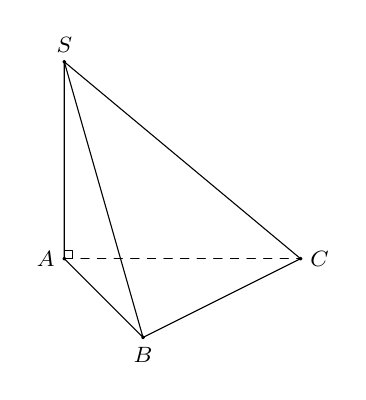
\begin{tikzpicture}[scale=0.5, font=\footnotesize, line join=round, line cap=round, >=stealth]
					%%%%%%%%%%%%%%%%%%%%%%%%%%%%%%%%%
					\coordinate (S) at (0,7);
					\coordinate (A) at (0,2);
					\coordinate (B) at (2,0);
					\coordinate (C) at (6,2);
					%%%%%%%%%%%%%%%%%%%%%%%%%%%%%%%%%
					\begin{scope}[dashed]
						\draw (A) -- (C);
					\end{scope}
					\draw (S) -- (A) -- (B) -- (C) -- (S) -- (B);
					\draw (A) rectangle (0.2,2.2);
					\filldraw [black] (0,7) circle (1pt) node[above] {$S$};
					\filldraw [black] (0,2) circle (1pt) node[left] {$A$};
					\filldraw [black] (2,0) circle (1pt) node[below] {$B$};
					\filldraw [black] (6,2) circle (1pt) node[right] {$C$};
					%%%%%%%%%%%%%%%%%%%%%%%%%%%%%%%%%
			\end{tikzpicture}}
		}
	\end{ex}
	
	\begin{ex}%[Đỗ Minh Phúc]%[1K7BO-2]%
		Cho hình chóp $S.ABCD$ có đáy $ABCD$ là hình thoi tâm $O$ và $SA=SC$, $SB=SD$. Mệnh đề nào sau đây \textbf{sai}?
		\choice
		{$SO \perp \left( ABCD \right)$}
		{$\left( SBD \right) \perp \left( ABCD \right)$}
		{\True $\left( SAB \right) \perp \left( SCB \right)$}
		{$\left( SAC \right) \perp \left( ABCD \right)$}
		\loigiai{
			\immini{
				Ta có $\Delta SAC$ cân (do $SA=SC$) có $SO$ là đường trung tuyến $\Rightarrow SO$ là đường cao $\Rightarrow SO \perp AC$.\\
				$\Delta SBD$ cân (do $SB=SD$) có $SO$ là đường trung tuyến $\Rightarrow SO$ là đường cao $\Rightarrow SO\perp BD$.\\
				Ta có
				$\left. \begin{aligned}
					& SO \perp AC \\
					& SO \perp BD \\
					& AC \cap BD=O \\
					& AC,BD \subset \left( ABCD \right) \\
				\end{aligned} \right\}\Rightarrow SO \perp \left( ABCD \right)$.\\
			}{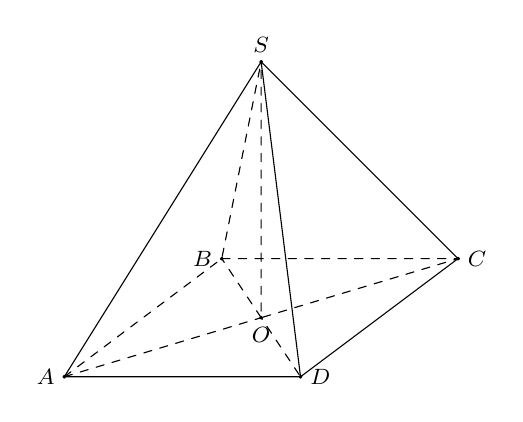
\begin{tikzpicture}[scale=0.5, font=\footnotesize, line join=round, line cap=round, >=stealth]
					%%%%%%%%%%%%%%%%%%%%%%%%%%%%%%%%%
					\coordinate (S) at (5,8);
					\coordinate (A) at (0,0);
					\coordinate (B) at (4,3);
					\coordinate (C) at (10,3);
					\coordinate (D) at (6,0);
					\coordinate (O) at (5,1.5);
					%%%%%%%%%%%%%%%%%%%%%%%%%%%%%%%%%
					\begin{scope}[dashed]
						\draw (A) -- (B) --(S); 
						\draw (B) -- (C) --(O)--(S); 
						\draw (A) -- (O) --(D); 
						\draw (O) --(B); 
					\end{scope}
					\draw (S) -- (A) -- (D) -- (C) -- (S) -- (D);
					%%%%%%%%%%%%%%%%%%%%%%%%%%%%%%%%%
					\filldraw [black] (5,8) circle (1pt) node[above] {$S$};
					\filldraw [black] (0,0) circle (1pt) node[left] {$A$};
					\filldraw [black] (4,3) circle (1pt) node[left] {$B$};
					\filldraw [black] (10,3) circle (1pt) node[right]{$C$};
					\filldraw [black] (6,0) circle (1pt) node[right]{$D$};
					\filldraw [black] (5,1.5) circle (1pt) node[below]{$O$};
					%%%%%%%%%%%%%%%%%%%%%%%%%%%%%%%%%
			\end{tikzpicture}}
			\noindent Mặt khác, $SO \subset \left( SAC \right)$, $SO\subset \left( SBD \right)$ $\Rightarrow \heva{&\left( SAC \right)\perp \left( ABCD \right) \\ &\left( SBD \right)\perp \left( ABCD \right).}$ 
		}
	\end{ex}
	
	\begin{ex}%[Đỗ Minh Phúc]%[1K7BO-7]%
		Cho hình chóp tam giác đều $S.ABC$ có $AB=a\sqrt{2}$. Mặt bên $\left( SBC \right)$ hợp với mặt đáy $\left( ABC \right)$ một góc $60^\circ$. Tính diện tích tam giác $SBC$.
		\choice
		{$\dfrac{a^2\sqrt{3}}{6}$}
		{$\dfrac{a^2\sqrt{2}}{3}$}
		{$\dfrac{a^2\sqrt{3}}{2}$}
		{\True $\dfrac{a^2\sqrt{3}}{3}$}
		\loigiai{
			\immini{
				Gọi $G$ là trọng tâm của tam giác $ABC$, vì $S.ABC$ là hình chóp tam giác đều nên $SG\perp \left( ABC \right)$.\\
				Ta có $ABC$ là tam giác đều có cạnh bằng $a\sqrt{2}$, gọi $AG \cap BC$ tại $D$, khi đó $AD\perp BC$ và $D$ là trung điểm của $BC$. \\
				Do đó $AD=\dfrac{a\sqrt{2} \cdot \sqrt{3}}{2}=\dfrac{a\sqrt{6}}{2}\Rightarrow GD=\dfrac{1}{3}AD=\dfrac{a\sqrt{6}}{6}$.\\
				Vì $S.ABC$ là hình chóp tam giác đều nên tam giác $SBC$ cân tại $S$, mà $D$ là trung điểm của $BC$ nên $SD \perp BC$. \\
				Ta có $AD\perp BC$, $SD\perp BC$. Vậy góc giữa hai mặt phẳng $\left( SBC \right)$ và $\left( ABC \right)$ bằng $\widehat{ADS}=60^\circ$.
			}{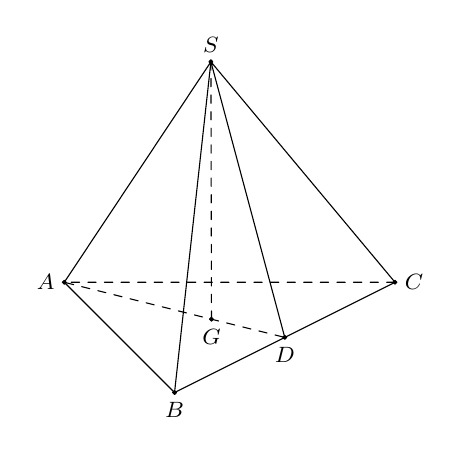
\begin{tikzpicture}[scale=0.7, font=\footnotesize, line join=round, line cap=round, >=stealth]
					%%%%%%%%%%%%%%%%%%%%%%%%%%%%%%%%%
					\coordinate (A) at (0,2);
					\coordinate (B) at (2,0);
					\coordinate (C) at (6,2);
					\coordinate (S) at (2.66,6);
					\coordinate (G) at (2.67,1.33);
					\coordinate (D) at (4,1);
					%%%%%%%%%%%%%%%%%%%%%%%%%%%%%%%%%
					\begin{scope}[dashed]
						\draw (S) -- (G);
						\draw (C) -- (A) -- (G) -- (D); 
					\end{scope}
					\draw (S) -- (A) --(B)--(D) -- (C) -- (S) -- (D);
					\draw (S) -- (B);
					%%%%%%%%%%%%%%%%%%%%%%%%%%%%%%%%%
					\filldraw [black] (0,2) circle (1pt) node[left] {$A$};
					\filldraw [black] (2,0) circle (1pt) node[below] {$B$};
					\filldraw [black] (6,2) circle (1pt) node[right] {$C$};
					\filldraw [black] (2.66,6) circle (1pt) node[above]{$S$};
					\filldraw [black] (2.67,1.33) circle (1pt) node[below] {$G$};
					\filldraw [black] (4,1) circle (1pt) node[below] {$D$};
					%%%%%%%%%%%%%%%%%%%%%%%%%%%%%%%%%
			\end{tikzpicture}}
			\noindent Xét tam giác $SGD$ vuông tại $G$, ta có $\cos \widehat{GDS}=\dfrac{GD}{SD} \Rightarrow SD=\dfrac{GD}{\cos \widehat{GDS}}=\dfrac{a\sqrt{6}}{6\cos 60^\circ}=\dfrac{a\sqrt{6}}{3}$.\\
			Vậy diện tích tam giác $SBC$ là $S_{SBC}=\dfrac{1}{2}SD \cdot BC=\dfrac{1}{2} \cdot \dfrac{a\sqrt{6}}{3} \cdot a\sqrt{2}=\dfrac{a^2\sqrt{3}}{3}$.
		}
	\end{ex}
	
	\begin{ex}%[Đỗ Minh Phúc]%[1K7BN-3]%
		Cho hình chóp $S.ABC$ có $SA$, $SB$, $SC$ đôi một vuông góc với nhau và $SA=SB=SC$. Gọi $I$ là trung điểm của $AB$. Tính góc giữa hai đường thẳng $SI$ và $BC$?
		\choice
		{$90^\circ$}
		{$120^\circ$}
		{\True $60^\circ$}
		{$30^\circ$}
		\loigiai{
			\immini{
				Gọi $J$ là trung điểm của $AC$ thì $IJ$ là đường trung bình của $\Delta ABC \Rightarrow IJ \parallel BC$.\\
				Vậy $\left(SI,BC \right)=\left( SI,IJ  \right)=\widehat{SIJ}$.\\
				Ta có $\Delta ABS$ vuông cân tại $S$ nên $SI=\dfrac{AB}{2}$.\\
				$\Delta ACS$ vuông cân tại $S$ nên $SJ=\dfrac{AC}{2}$.\\
				$IJ$ là đường trung bình của $\Delta ABC\Rightarrow IJ=\dfrac{1}{2}BC$. \\ 
				Mà $SA=SB=SC \Rightarrow AB=AC=BC$. Suy ra $SI=SJ=IJ\Rightarrow \Delta SIJ$ đều. \\ 
				Suy ra $\widehat{SIJ}=60^\circ$. 
			}{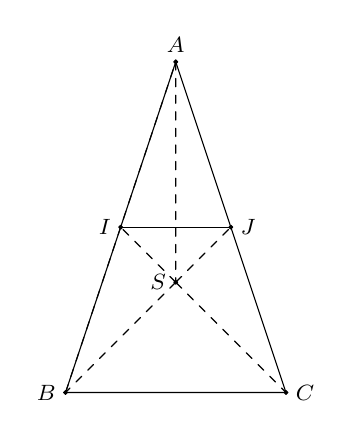
\begin{tikzpicture}[scale=0.7, font=\footnotesize, line join=round, line cap=round, >=stealth]
					%%%%%%%%%%%%%%%%%%%%%%%%%%%%%%%%%
					\coordinate (A) at (0,6);
					\coordinate (S) at (0,2);
					\coordinate (B) at (-2,0);
					\coordinate (C) at (2,0);
					\coordinate (I) at (-1,3);
					\coordinate (J) at (1,3);
					%%%%%%%%%%%%%%%%%%%%%%%%%%%%%%%%%
					\begin{scope}[dashed]
						\draw (B) -- (A)-- (S);
						\draw (S) -- (I);
						\draw (S) -- (J);
						\draw (S) -- (C);
						\draw (S) -- (B);
					\end{scope}
					\draw (B) -- (I) -- (A) --(J) --  (C) -- (B);
					\draw (I) -- (J);
					%%%%%%%%%%%%%%%%%%%%%%%%%%%%%%%%%
					\filldraw [black] (0,6) circle (1pt) node[above] {$A$};
					\filldraw [black] (0,2) circle (1pt) node[left] {$S$};
					\filldraw [black] (-2,0) circle (1pt) node[left] {$B$};
					\filldraw [black] (2,0) circle (1pt) node[right] {$C$};
					\filldraw [black] (-1,3) circle (1pt) node[left] {$I$};
					\filldraw [black] (1,3) circle (1pt) node[right] {$J$};
					%%%%%%%%%%%%%%%%%%%%%%%%%%%%%%%%%
			\end{tikzpicture}}
		}
	\end{ex}
	
	\begin{ex}%[Đỗ Minh Phúc]%[1K7BM-2]%
		Cho tứ diện $ABCD$, biết $\triangle ABC$ và $\triangle BCD$ là hai tam giác cân có chung cạnh đáy $BC$. Gọi $H$ là trung điểm của cạnh $BC$. Khẳng định nào đúng trong các khẳng định sau
		\choice
		{$AC \perp(ADH)$}
		{$BC \parallel(ADH)$}
		{$AB \perp(ADH)$}
		{\True $BC \perp(ADH)$}
		\loigiai{
			\immini{Ta có $\heva{&BC\perp AH\\&BC\perp DH}\Rightarrow BC\perp(ADH)$.}{\begin{tikzpicture}[scale=0.7, font=\footnotesize, line join=round, line cap=round, >=stealth]
					\coordinate (B)at (0,0);
					\coordinate (D)at (5,0);
					\coordinate (C) at (2,-2);
					\coordinate (A) at (3,3);
					\coordinate (H) at ($(B)!.5!(C)$); 
					\foreach \x/\g in {A/160,B/180,C/-90,D/0,H/200} \fill (\x) circle (1pt) +(\g:3mm) node{$\x$};
					\draw (H)--(A)--(B)--(C)--(D)--(A)--(C);
					\draw[dashed] (B)--(D)--(H);
					\foreach \x in {A,B,C,D,H}	\fill(\x)circle(1.5pt);
			\end{tikzpicture}}
		}
	\end{ex}
	
	\begin{ex}%[Đỗ Minh Phúc]%[1K7KN-3]%
		Cho hình chóp $S.ABCD$ có đáy $ABCD$ là hình vuông cạnh $a$, cạnh bên $SA$ vuông góc với mặt đáy và $SA=a \sqrt{2}$. Tìm số đo của góc giữa đường thẳng $SC$ và mặt phẳng $(SAD)$.
		\choice
		{$45^{\circ}$}
		{$60^{\circ}$}
		{$90^{\circ}$}
		{\True $30^{\circ}$}
		\loigiai{
			\immini{Ta có $\heva{&CD\perp SA\\&CD\perp AD}\Rightarrow CD\perp(SAD)$.\\
				Khi đó $SD$ là hình chiếu vuông góc của $SC$ lên mặt phẳng $(SAD)$.\\
				Suy ra góc giữa đường thẳng $SC$ và mặt phẳng $(SAD)$ là $\widehat{CSD}$ (vì tam giác $SCD$ vuông tại $D$).\\
				Trong tam giác $SAD$ ta có $$SD=\sqrt{SA^2+AD^2}=\sqrt{\left(a\sqrt{2}\right)^2+a^2}=a\sqrt{3}.$$
				Trong tam giác $SCD$ ta có
				$$\tan\widehat{CSD}=\dfrac{CD}{SD}=\dfrac{a}{a\sqrt{3}}=\dfrac{1}{\sqrt{3}}\Rightarrow\widehat{CSD}=30^\circ.$$
			}{\begin{tikzpicture}[scale=1, font=\footnotesize, line join=round, line cap=round, >=stealth]
					\coordinate (A)at (0,0);
					\coordinate (B)at (-2,-2);
					\coordinate (D) at (5,0);
					\coordinate (C) at ($(B)-(A)+(D)$);
					\coordinate (S) at ($(A)+(90:4)$);
					\foreach \x/\g in {A/160,B/180,C/-45,D/0,S/90} \fill (\x) circle (1pt) +(\g:3mm) node{$\x$};
					\draw (S)--(B)--(C)--(S)--(D)--(C)node[right,midway]{$a$};
					\draw[dashed] (S)--(A)node[right,midway]{$a\sqrt{2}$}--(B) (D)--(A)node[above right,midway]{$a$};
					\foreach \x in {A,B,C,D,S}	\fill (\x)circle(1.5pt);
			\end{tikzpicture}}
		}
	\end{ex}
	
	\begin{ex}%[Đỗ Minh Phúc]%[1K7BO-3]%
		Cho hình chóp tứ giác đều $S.ABCD$ có cạnh đáy bằng $2a$ và chiều cao bằng $a\sqrt{3}$, số đo góc giữa mặt bên và mặt đáy bằng
		\choice
		{\True $60^{\circ}$}
		{$45^{\circ}$}
		{$30^{\circ}$}
		{$75^{\circ}$}
		\loigiai{
			\immini{
				Gọi $M$ là trung điểm của $BC$, góc giữa mặt $(SBC)$ và $(ABCD)$ là $\alpha=\widehat{SMO}$.\\
				Ta có $\tan \alpha=\dfrac{SO}{OM}=\dfrac{\sqrt{3}}{1}\Rightarrow\alpha =60^\circ$.
			}{
				\begin{tikzpicture}[font=\footnotesize, line join=round, line cap=round, >=stealth]%Choptugiacdeu
					\def\a{1.75}
					\def\b{0.75*\a}
					\path(0,0) coordinate(A)(\a,0)coordinate(B)(-135:\b)coordinate(D)++(0:\a)coordinate(C)($(A)!0.5!(C)$)coordinate(O)++(90:1.25*\a)coordinate(S)($(C)!0.5!(B)$)coordinate(M);
					\draw[dotted](S)--(A)--(B)(D)--(A)(S)--(O)--(M)(A)--(C)(B)--(D);
					\draw(S)--(D)--(C)--(B)--(S)(S)--(C)(S)--(M);
					\foreach \d/\g in{A/180,B/0,C/-90,D/-90,S/90,O/-90,M/0}
					\draw[fill=black](\d)circle(1pt)node[shift={(\g:0.25)}]{$\d$};
				\end{tikzpicture}
			}	
		}
	\end{ex}
	
	\begin{ex}%[Đỗ Minh Phúc]%[1K7BN-3]%
		Cho hình chóp đều $S.ABCD$. Góc giữa các cạnh bên và mặt phẳng đáy là góc nào sau đây?
		\choice
		{\True $\widehat{SAC}$}
		{$\widehat{SAB}$}
		{$\widehat{SAD}$}
		{$\widehat{BAD}$}
		\loigiai{
			\immini{Góc giữa cạnh bên và mặt đáy là các góc $\widehat{SCA}$, $\widehat{SAC}$, $\widehat{SBD}$, $\widehat{SDB}$.}{
				\begin{tikzpicture}[font=\footnotesize, line join=round, line cap=round, >=stealth]%Choptugiacdeu
					\def\a{2}
					\def\b{0.5*\a}
					\path(0,0) coordinate(A)(\a,0)coordinate(B)(-135:\b)coordinate(D)++(0:\a)coordinate(C)($(A)!0.5!(C)$)coordinate(O)++(90:\a)coordinate(S);
					\draw[dotted](S)--(A)--(B)(D)--(A)(S)--(O)(A)--(C)(B)--(D);
					\draw(S)--(D)--(C)--(B)--(S)(S)--(C);
					\foreach \d/\g in{A/180,B/0,C/-90,D/-90,S/90,O/-90}
					\draw[fill=black](\d)circle(1pt)node[shift={(\g:0.25)}]{$\d$};
				\end{tikzpicture}		
			}		
		}
	\end{ex}
	
	\begin{ex}%[Đỗ Minh Phúc]%[1K7BN-3]%
		\immini{
			Cho hình chóp $S.ABCD$, đáy $ABCD$ là hình chữ nhật có cạnh $AB=a$, $BC=2a$. Cạnh bên $SA$ vuông góc với mặt phẳng đáy $(ABCD)$ và $SA=a\sqrt{15}$. Tính góc tạo bởi đường thẳng $SC$ và mặt phẳng $(ABCD)$.
			\choice
			{$45^{\circ}$}
			{$90^{\circ}$}
			{\True $60^{\circ}$}
			{$30^{\circ}$}
		}{
			\begin{tikzpicture}[scale=0.7, font=\footnotesize, line join=round, line cap=round,>=stealth]
				\path
				(0,0) coordinate (A)
				(-1.3,-1.6) coordinate (B)
				(2.5,-1.6)coordinate (C)
				($(A)+(C)-(B)$) coordinate (D)
				($(A)+(0,3)$) coordinate (S)
				;
				\draw (S)--(B)--(C)--(D)--cycle (S)--(C);
				\draw[dashed] (S)--(A)--(D) (A)--(B);	
				\foreach \p/\q in {S/90,A/-90,B/-90,C/-90,D/0}			
				\fill[black] (\p) circle (1.0pt)node[shift={(\q:2.5mm)}]{$\p$};
			\end{tikzpicture}
		}
		\loigiai{
			\immini{
				Vì $SA\perp(ABCD)$ nên hình chiếu vuông góc của $SC$ trên $(ABCD)$ là $AC$.\\
				Do đó $\left(SC,(ABCD)\right)=(SC,AC)=\widehat{SCA}$.\\
				Trong tam giác $SAC$ vuông tại $A$, ta có \[\tan\widehat{SCA}=\dfrac{SA}{AC}=\dfrac{SA}{\sqrt{AB^2+BC^2}}=\dfrac{a\sqrt{15}}{\sqrt{a^2+(2a^2)}}=\sqrt{3}.\]
				Suy ra $\widehat{SCA}=60^\circ$ hay $\left(SC,(ABCD)\right)=60^\circ$.
			}{
				\begin{tikzpicture}[scale=0.7, font=\footnotesize, line join=round, line cap=round,>=stealth]
					\path
					(0,0) coordinate (A)
					(-1.3,-1.6) coordinate (B)
					(2.5,-1.6)coordinate (C)
					($(A)+(C)-(B)$) coordinate (D)
					($(A)+(0,3)$) coordinate (S)
					;
					\draw (S)--(B)--(C)--(D)--cycle (S)--(C);
					\draw[dashed] (S)--(A)--(D) (C)--(A)--(B);	
					\foreach \p/\q in {S/90,A/-90,B/-90,C/-90,D/0}			
					\fill[black] (\p) circle (1.0pt)node[shift={(\q:2.5mm)}]{$\p$};
				\end{tikzpicture}
			}		
		}
	\end{ex}
	
	\begin{ex}%[Đỗ Minh Phúc]%[1K7BM-2]%
		Cho hình lập phương $ABCD.A'B'C'D'$. Đường thẳng $AC'$ vuông góc với mặt phẳng nào sau đây?
		\choice
		{$AC'\perp(BB'D'D)$}
		{$AC'\perp(ABCD)$}
		{$AC'\perp(AA'D'D)$}
		{\True $AC'\perp(A'BD)$}
		\loigiai{
			\immini{
				Hình chiếu vuông góc của $AC'$ trên $(ABCD)$ là $AC$.\\
				Mặt khác $AC\perp BD$ nên $AC'\perp BD$.\\
				Chứng minh tương tự ta cũng có $AC'\perp A'D$.\\
				Vậy $\heva{& AC'\perp BD \\ & AC'\perp A'D}\Rightarrow AC'\perp(A'BD)$.
			}{
				\begin{tikzpicture}[scale=0.7,font=\footnotesize,line join=round,line cap=round,>=stealth]
					\path
					(0,0) coordinate (B)
					(1,0.8) coordinate (A)
					(4,0) coordinate (C)
					($(C)-(B)+(A)$) coordinate (D)	
					($(A)+(90:3.5)$) coordinate (A')
					($(B)-(A)+(A')$) coordinate (B')
					($(C)-(A)+(A')$) coordinate (C')
					($(D)-(A)+(A')$) coordinate (D')
					;
					\draw (B')--(B)--(C)--(D)--(D')--(A')--(B')--(C')--(D') (C)--(C');
					\draw[dashed] (C')--(A)--(D)--(B) (A')--(A)--(B)--cycle (D)--(A');
					\foreach \p/\q in {A/160,B/-135,C/-45,D/0,A'/90,B'/180,C'/-20,D'/0}
					\fill[black] (\p)node[shift={(\q:3mm)}]{$\p$} circle (1.0pt);	
				\end{tikzpicture}
			}
		}
	\end{ex}
	
	\begin{ex}%[Đỗ Minh Phúc]%[1K7BM-4]%
		\immini{
			Cho hình chóp $S.ABCD$ có đáy là hình vuông và cạnh bên $SA$ vuông góc với mặt phẳng đáy $(ABCD)$ (minh họa như hình bên). Trong các mệnh đề sau, mệnh đề nào \textbf{sai}?
			\choice
			{$SA\perp AB$}
			{$AC\perp BD$}
			{\True $AC\perp SB$}
			{$SA\perp AD$}
		}{
			\begin{tikzpicture}[scale=0.7, font=\footnotesize, line join=round, line cap=round,>=stealth]
				\path
				(0,0) coordinate (A)
				(-1.3,-1.6) coordinate (B)
				(2.5,-1.6)coordinate (C)
				($(A)+(C)-(B)$) coordinate (D)
				($(A)+(0,3)$) coordinate (S)
				;
				\draw (S)--(B)--(C)--(D)--cycle (S)--(C);
				\draw[dashed] (S)--(A)--(D) (A)--(B);	
				\foreach \p/\q in {S/90,A/-90,B/-90,C/-90,D/0}			
				\fill[black] (\p) circle (1.0pt)node[shift={(\q:2.5mm)}]{$\p$};
			\end{tikzpicture}
		}
		\loigiai{
			Vì $SA\perp (ABCD)\Rightarrow\heva{& SA\perp AB \\ & SA\perp AD}$ suy ra mệnh đề \lq\lq $SA\perp AB$\rq\rq, \lq\lq $SA\perp AD$\rq\rq\, đúng.\\
			Mặt khác $ABCD$ là hình vuông nên $AC\perp BD$ do đó mệnh đề \lq\lq $AC\perp BD$\rq\rq\, đúng.
		}
	\end{ex}
	
	\begin{ex}%[Đỗ Minh Phúc]%[1K7BM-2]%
		\immini{
			Cho hình chóp $S.ABC$ có đáy $ABC$ là tam giác đều, cạnh bên $SA\perp(ABC)$. Gọi $M$ là trung điểm cạnh $BC$. Khẳng định nào trong các khẳng định sau là khẳng định đúng?
			\choice
			{\True $BC\perp(SAM)$}
			{$BC\perp(SAC)$}
			{$AM\perp(SBC)$}
			{$AC\perp(SBC)$}
		}{
			\begin{tikzpicture}[scale=0.7, font=\footnotesize, line join=round, line cap=round,>=stealth]
				\path
				(0,0) coordinate (A)
				(1.2,-1.4) coordinate (B)
				(4,0) coordinate (C)
				($(A)+(0,3)$) coordinate (S)
				($(C)!0.5!(B)$) coordinate (M)				
				;
				\draw (S)--(A)--(B)--(C)--cycle (M)--(S)--(B);	
				\draw[dashed] (M)--(A)--(C);	
				\foreach \p/\q in {S/90,A/180,B/-90,C/0,M/-60}
				\fill[black] (\p) circle (1.0pt) ($(\p)+(\q:2.5mm)$) node{$\p$};
			\end{tikzpicture}
		}
		\loigiai{
			Vì $\heva{& SA\perp(ABC) \\ & BC\subset(ABC)}\Rightarrow SA\perp BC.\quad(1)$\\
			Mặt khác $\triangle ABC$ đều suy ra $BC\perp AM.\quad(2)$\\
			Từ $(1)$ và $(2)$ suy ra $BC\perp(SAM)$.
		}
	\end{ex}
	
	\begin{ex}%[Đỗ Minh Phúc]%[1K7BM-4]%
		\immini{
			Cho hình chóp $S.ABCD$ có đáy $ABCD$ là hình chữ nhật, $SA\perp(ABCD)$, $AH\perp SB$ tại $H$. Khi đó $AH$ vuông góc được với đường thẳng nào sau đây?
			\choice
			{$BD$}
			{$SD$}
			{$CD$}
			{\True $SC$}
		}{
			\begin{tikzpicture}[scale=0.7, font=\footnotesize, line join=round, line cap=round,>=stealth]
				\path
				(0,0) coordinate (A)
				(-1.3,-1.6) coordinate (B)
				(2.5,-1.6)coordinate (C)
				($(A)+(C)-(B)$) coordinate (D)
				($(A)+(0,3)$) coordinate (S)
				($(S)!0.55!(B)$) coordinate (H)			
				;
				\draw (S)--(B)--(C)--(D)--cycle (S)--(C);
				\draw[dashed] (S)--(A)--(D) (H)--(A)--(B);	
				\foreach \p/\q in {S/90,A/-90,B/-90,C/-90,D/0,H/180}			
				\fill[black] (\p) circle (1.0pt)node[shift={(\q:2.5mm)}]{$\p$};
			\end{tikzpicture}
		}
		\loigiai{
			Vì $\heva{& SA\perp(ABCD) \\ & BC\subset(ABCD)}\Rightarrow SA\perp BC.\quad(1)$\\
			Ta có $BC\perp AB.\quad(2)$\\
			Từ $(1)$ và $(2)$ suy ra $BC\perp(SAB)\Rightarrow BC\perp AH.\quad(3)$\\
			Mặt khác $AH\perp SB.\quad(4)$\\
			Từ $(3)$ và $(4)$ suy ra $AH\perp(SBC)\Rightarrow AH\perp SC$.
		}
	\end{ex}
	
	\begin{ex}%[Đỗ Minh Phúc]%[1K7BP-3]%
		Cho hình chóp $S.ABC$ có đáy là tam giác vuông tại $B$. Biết $SA$ vuông góc với mặt phẳng đáy, $SA=AB=a\sqrt{3}$. Khoảng cách từ điểm $A$ tới mặt phẳng $(SBC)$ là
		\choice
		{\True $\dfrac{a\sqrt{6}}{2}$}
		{$a\sqrt{3}$}
		{$a\sqrt{6}$}
		{$\dfrac{a\sqrt{6}}{3}$}
		\loigiai{
			\immini{
				Gọi $H$ là trung điểm của $SB$, suy ra $AH\perp SB$ (do $\triangle SAB$ cân tại $A$).\\
				Ta có $\heva{& BC\perp SA \\ & BC\perp AB}\Rightarrow BC\perp (SAB)$.\\
				Do đó $\heva{& AH\perp SB \\ & AH\perp BC}\Rightarrow AH\perp(SBC)$.\\
				Vậy $\mathrm{d}\left(A,(SBC)\right)=AH=\dfrac{SC}{2}=\dfrac{\sqrt{SA^2+AB^2}}{2}=\dfrac{a\sqrt{6}}{2}$.
			}{
				\begin{tikzpicture}[scale=1, font=\footnotesize, line join=round, line cap=round,>=stealth]
					\path
					(0,0) coordinate (A)
					(1.2,-1.5) coordinate (B)
					(4,0) coordinate (C)
					($(A)+(0,3.3)$) coordinate (S)
					($(S)!0.5!(B)$) coordinate (H)				
					;
					\draw (S)--(A)--(B)--(C)--cycle (S)--(B) (A)--(H);	
					\draw[dashed] (A)--(C);	
					\foreach \p/\q in {S/90,A/180,B/-90,C/0,H/10}
					\fill[black] (\p) circle (1.0pt) ($(\p)+(\q:2.5mm)$) node{$\p$};
					%\tkzMarkRightAngles(S,A,C A,B,C A,H,B)
				\end{tikzpicture}
			}
		}
	\end{ex}
	
	\begin{ex}%[Đỗ Minh Phúc]%[1K7BO-3]%
		Cho hình chóp $S.ABCD$ có đáy là hình vuông và cạnh bên $SA$ vuông góc với mặt phẳng đáy $(ABCD)$. Góc giữa mặt phẳng $(SBC)$ và mặt phẳng đáy $(ABCD)$ là góc nào sau đây?
		\choice
		{$\widehat{SAB}$}
		{\True $\widehat{SBA}$}
		{$\widehat{SBC}$}
		{$\widehat{SBD}$}
		\loigiai{
			\immini{
				Ta có $\heva{& BC\perp SA \\ & BC\perp AB}\Rightarrow BC\perp SB$.\\
				Vì $\heva{& (SBC)\cap(ABCD)=BC \\ & SB\perp BC,SB\subset(SAB)\\ &AB\perp BC,AB\subset(ABCD)}$ nên $\left((SBC),(ABCD)\right)=(SB,AB)=\widehat{SBA}$.
			}{
				\begin{tikzpicture}[scale=0.8, font=\footnotesize, line join=round, line cap=round,>=stealth]
					\path
					(0,0) coordinate (A)
					(-1.3,-1.6) coordinate (B)
					(2.5,-1.6)coordinate (C)
					($(A)+(C)-(B)$) coordinate (D)
					($(A)+(0,3)$) coordinate (S)
					;
					\draw (S)--(B)--(C)--(D)--cycle (S)--(C);
					\draw[dashed] (S)--(A)--(D) (A)--(B);	
					\foreach \p/\q in {S/90,A/-90,B/-90,C/-90,D/0}			
					\fill[black] (\p) circle (1.0pt)node[shift={(\q:2.5mm)}]{$\p$};
					%\tkzMarkRightAngles(S,A,B S,A,D)
				\end{tikzpicture}
			}
		}
	\end{ex}
	
	\begin{ex}%[Đỗ Minh Phúc]%[1K7KP-4]%
		Cho hình chóp $S.ABCD$ có đáy $ABCD$ là hình vuông, biết $AC=\dfrac{\sqrt{2}a}{2}$, $SA$ vuông góc với đáy, $SB$ tạo với đáy một góc $60^\circ$. Khoảng cách giữa $AD$ và $SC$ bằng
		\choice
		{$\dfrac{\sqrt{2}a}{2}$}
		{$\dfrac{\sqrt{3}a}{2}$}
		{$\dfrac{a}{3}$}
		{\True $\dfrac{\sqrt{3}a}{4}$}
		\loigiai{
			\immini{
				Do $ABCD$ là hình vuông nên $AB=AC\cdot\dfrac{\sqrt{2}}{2}=\dfrac{a}{2}$.\\
				Do $AD\parallel (SBC)\Rightarrow \mathrm{d}\left(AD,(SBC)\right)=\mathrm{d}\left(A,(SBC)\right)$.\\
				Gọi $H$ là hình chiếu vuông góc của $A$ lên $SB$.\\
				Ta có $\heva{&AH\perp SB\\&AH\perp BC\,(\text{Do $BC\perp (SAB)$})}\Rightarrow AH\perp (SBC)$.\\
				Suy ra $\mathrm{d}\left(AD,SC\right)=AH=AB\cdot \sin 60^\circ=\dfrac{a}{2}\cdot\dfrac{\sqrt{3}}{2}=\dfrac{\sqrt{3}}{4}a$.
			}
			{
				\begin{tikzpicture}[font=\footnotesize, line join=round, line cap=round, >=stealth]
					\def\a{2}
					\path(0,0)coordinate(A)(\a,0)coordinate(B)(-135:0.5*\a)coordinate(D)++(0:\a)coordinate(C)(90:\a)coordinate(S)($(S)!(A)!(B)$)coordinate(H);
					\draw(S)--(D)--(C)--(B)--(S)--(C);
					\draw[dotted](D)--(A)--(B)--(D)(S)--(A)--(H);
					\foreach \d/\g in{A/180,S/90,B/0,C/-90,D/-90,H/30}
					\draw[fill=black](\d)circle(1pt)node[shift={(\g:0.25)}]{$\d$};
				\end{tikzpicture}
			}
		}
	\end{ex}
	
	\begin{ex}%[Đỗ Minh Phúc]%[1K7KL-2]%
		Cho hình chóp $S.ABC$ có đáy $ABC$ là tam giác vuông tại $B$, $AB=2a$, $BC=2 a\sqrt{3}$. Biết rằng mặt bên $(SAB)$ là tam giác đều và nằm trong mặt phẳng vuông góc với mặt đáy $(ABC)$. Gọi $M$ là trung điểm của $BC$. Cô-sin của góc giữa hai đường thẳng $SC$ và $AM$ bằng
		\choice
		{$\dfrac{4}{7}$}
		{$\dfrac{1}{\sqrt{7}}$}
		{\True $\dfrac{2}{\sqrt{7}}$}
		{$\dfrac{2}{7}$}
		\loigiai{
			\immini{
				Từ giả thiết suy ra $SH=\sqrt{3}a$, $AC=4a$, $HC=\sqrt{13}a$, $SC=4a$.\\
				Gọi $N$ là trung điểm của $SB\Rightarrow MN\parallel SC\Rightarrow$ ta có
				\[\cos\left(SC,AM\right)=\cos\left(AM,MN\right)=\left|\dfrac{MA^2+MN^2-AN^2}{2AM\cdot MN}\right|\quad(1).\]
				Ta có $AM=\sqrt{BM^2+AB^2}=\sqrt{4a^2+3a^2}=\sqrt{7}a$, $MN=2a$, $AN=\sqrt{3}a$.	\\
				Thế vào $(1)$ ta được $\cos\left(SC,AM\right)=\dfrac{7a^2+4a^2-3a^2}{2\sqrt{7}a\cdot 2a}=\dfrac{2}{\sqrt{7}}$.
			}{
				\begin{tikzpicture}[font=\footnotesize, line join=round, line cap=round, >=stealth]%Hinhchop
					\def\a{2}
					\def\b{0.8*\a}
					\path(0,0)coordinate(A)++(\a,0)coordinate(B)++(-145:\b)coordinate(C)(0.5*\a,0)coordinate(H)++(90:\a)coordinate(S)(C)($(B)!0.5!(C)$)coordinate(M)($(B)!0.5!(S)$)coordinate(N);
					\draw[dotted](A)--(B)(S)--(H)(A)--(M)(A)--(N);
					\draw(S)--(C)(S)--(A)--(C)(B)--(S)(C)--(B)(M)--(N);
					\foreach \d/\g in{A/180,C/-90,B/0,S/90,H/45,M/-40,N/45}
					\draw[fill=black](\d) circle(1pt)node[shift={(\g:0.25)}]{$\d$};
				\end{tikzpicture}
			}
			Vậy cosin của góc tạo bởi $SC$ và $AM$ bằng $\dfrac{2}{\sqrt{7}}$.
		}
	\end{ex}
	
	\begin{ex}%[Đỗ Minh Phúc]%[1K7BP-3]%
		Cho hình chóp $S.ABCD$ có đáy $ABCD$ là hình vuông cạnh $a\sqrt{2}$, cạnh $SA=a$ và $SA \perp \left( ABCD \right)$. Khoảng cách từ điểm $A$ đến mặt phẳng $\left( SBD \right)$ bằng
		\choice
		{\True $\dfrac{a\sqrt{2}}{2}$}
		{$a\sqrt{2}$}
		{$\dfrac{a\sqrt{3}}{2}$}
		{$2a$}
		\loigiai{
			\immini{
				Gọi $O$ là giao điểm của $AC$ và $BD$. Kẻ $AH \perp SO$ tại $H$. \\  
				Ta có \\ 
				$\heva{
					& AC\perp BD  \text{ vì $ABCD$ là hình vuông}\\
					& SA \perp BD \text{ vì $SA \perp ABCD$} \\
					& SA \cap AC=A \\
					& SA, AC \subset \left( SAC \right)} \Rightarrow BD \perp \left( SAC \right)\Rightarrow BD\perp AH$. \\ 
				Mặt khác \\ 
				$\heva{
					& AH \perp SO  \\
					& AH \perp BD  \\
					& SO \cap BD=O \\
					& SO,BD\subset \left( SBD \right)} \Rightarrow AH \perp \left( SBD \right) \Rightarrow \mathrm{d} \left( A,(SBD) \right)=AH$. 
			}{
				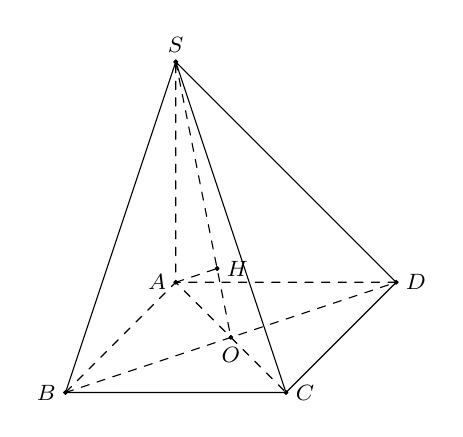
\begin{tikzpicture}[scale=0.7, font=\footnotesize, line join=round, line cap=round, >=stealth]
					%%%%%%%%%%%%%%%%%%%%%%%%%%%%%%%%%
					\coordinate (S) at (0,6);
					\coordinate (A) at (0,2);
					\coordinate (B) at (-2,0);
					\coordinate (C) at (2,0);
					\coordinate (D) at (4,2);
					\coordinate (O) at (1,1);
					\coordinate (H) at (0.75,2.25);
					%%%%%%%%%%%%%%%%%%%%%%%%%%%%%%%%%
					\begin{scope}[dashed]
						\draw (B) -- (A)-- (S);
						\draw (D) -- (A) -- (C);
						\draw (B) -- (D);
						\draw (A) -- (H);
						\draw (S) -- (O);
					\end{scope}
					\draw (S) -- (B) -- (C) -- (D) -- (S) -- (C);
					%%%%%%%%%%%%%%%%%%%%%%%%%%%%%%%%%
					\filldraw [black] (0,6) circle (1pt) node[above] {$S$};
					\filldraw [black] (0,2) circle (1pt) node[left]{$A$};
					\filldraw [black] (-2,0) circle (1pt) node[left] {$B$};
					\filldraw [black] (2,0) circle (1pt) node[right] {$C$};
					\filldraw [black] (4,2) circle (1pt) node[right]{$D$};
					\filldraw [black] (1,1) circle (1pt) node[below]{$O$};
					\filldraw [black] (0.75,2.25) circle (1pt) node[right]{$H$};
					%%%%%%%%%%%%%%%%%%%%%%%%%%%%%%%%%
			\end{tikzpicture}} 
			\noindent Xét tam giác $SAO$ vuông tại $A$, $AH \perp SO$ nên ta có $\dfrac{1}{AH^2}=\dfrac{1}{SA^2}+\dfrac{1}{AO^2}=\dfrac{1}{a^2}+\dfrac{1}{a^2}=\dfrac{2}{a^2} \Rightarrow AH=\dfrac{a\sqrt{2}}{2}$.
		}
	\end{ex}
	
	\begin{ex}%[Đỗ Minh Phúc]%[1K7BP-3]%
		Cho hình lập phương $ABCD.A'B'C'D'$ có cạnh bằng $2$. Khoảng cách từ điểm $D$ đến mặt phẳng $(ACD')$ là
		\choice
		{$2\sqrt{2}$}
		{\True $\dfrac{2 \sqrt{3}}{3}$}
		{$\dfrac{2 \sqrt{6}}{3}$}
		{Đáp án khác}
		\loigiai{
			\immini{Gọi $O$ là tâm của hình vuông $ABCD$ và $H$ là hình chiếu vuông góc của $D$ lên $D'O$.\\
				Ta có $\heva{&AC\perp DO\\&AC\perp D'D}\Rightarrow AC\perp(D'OD)\Rightarrow AC\perp DH$.\\
				Khi đó $\heva{&DH\perp AC\\&DH\perp D'O}\Rightarrow DH\perp\left( ACD'\right) \Rightarrow\mathrm{d}\left( D,(ACD')\right) =DH$.\\
				Vì $ABCD.A'B'C'D'$ là hình lập phương cạnh bằng $2$ nên\\  $BD=2\sqrt{2}\Rightarrow DO=\sqrt{2}$.\\
				Trong tam giác $D'DO$ ta có
				$$\dfrac{1}{DH^2}=\dfrac{1}{DO^2}+\dfrac{1}{DD'^2}=\dfrac{1}{\left( \sqrt{2}\right) ^2}+\dfrac{1}{2^2}=\dfrac{3}{4}\Rightarrow DH=\dfrac{2 \sqrt{3}}{3}.$$}{\begin{tikzpicture}[scale=0.8, font=\footnotesize, line join=round, line cap=round, >=stealth]
					\coordinate (A)at (0,0);
					\coordinate (B)at (-2,-2);
					\coordinate (D) at (5,0);
					\coordinate (C) at ($(B)-(A)+(D)$);
					\coordinate (A') at ($(A)+(90:4)$);
					\coordinate (B') at ($(B)+(90:4)$);
					\coordinate (C') at ($(C)+(90:4)$);
					\coordinate (D') at ($(D)+(90:4)$);
					\coordinate (O) at ($(A)!.5!(C)$);
					\coordinate (H) at ($(D')!.4!(O)$); 
					\newcommand{\gocv}[4][black]{\draw[#1] ($(#3)!5pt!(#2)$)--($(#3)!2!($($(#3)!5pt!(#2)$)!.5!($(#3)!5pt!(#4)$)$)$)--($(#3)!5pt!(#4)$);}
					\gocv{D}{H}{D'}
					\foreach \x/\g in {A/160,B/180,C/-45,D/0,A'/90,B'/180,C'/-130,D'/0,O/-90,H/190} \fill (\x) circle (1pt) +(\g:3mm) node{$\x$};
					\draw (B')--(B)--(C)--(D)--(D')--(C')--(B')--(A')--(D')--(C) (C)--(C');
					\draw[dashed] (B)--(D)--(A)--(A') (B)--(A)--(C) (A)--(D')--(O) (D)--(H);
					\foreach \x in {A,B,C,D,A',B',C',D',O}	\fill(\x)circle(1.5pt);
			\end{tikzpicture}}
		}
	\end{ex}
	
	\begin{ex}%[Đỗ Minh Phúc]%[1K7KP-4]%
		Cho hình chóp $S.ABCD$ có đáy là hình bình hành thỏa mãn $SA=SB=SC=22$, $\widehat{SBC}=30^{\circ}$, $\widehat{SAB}=60^{\circ}$ và $\widehat{SCA}=45^{\circ}$. Khoảng cách giữa hai đường thẳng $AB$ và $SD$ là
		\choice
		{$2\sqrt{22}$}
		{$4\sqrt{11}$}
		{$\dfrac{\sqrt{22}}{2}$}
		{\True Đáp án khác}
		\loigiai{
			\immini{Do $SA=SB=22$ và $\widehat{SAB}=60^{\circ}$ nên $\triangle SAB$ đều $\Rightarrow AB=22$.\\
				Do $SA=SC=22$ và $\widehat{SCA}=45^{\circ}$ nên $\triangle ASC$ vuông tại $S$ $\Rightarrow AC=22 \sqrt{2}$.\\
				$\triangle SBC$ có $SB=SC=22$, $\widehat{SBC}=30^{\circ}$.\\
				$SC^{2}=SB^{2}+BC^{2}-2 SB \cdot BC \cdot \cos \widehat{SBC} \Rightarrow BC=22 \sqrt{3}$.\\
				Do $BC^{2}=AB^{2}+AC^{2} \Rightarrow \triangle ABC$ vuông tại $A$.\\
				Gọi $H$ là trung điểm của $BC \Rightarrow H$ là tâm đường tròn ngoại tiếp $\triangle ABC$.\\
				Do $SA=SB=SC$ nên $SH \perp(ABC)$.\\
				$SH=\sqrt{SC^{2}-HC^{2}}=\sqrt{22^{2}-(11 \sqrt{3})^{2}}=11$.\\
				Trong $(ABCD)$, gọi $K$, $L$ lần lượt là hình chiếu vuông góc của $H$, $B$ trên $CD$, khi đó $HK\parallel BL$ và $HK=\dfrac{1}{2} BL=\dfrac{1}{2} AC=11 \sqrt{2}$.\\
				Trong $(SHK)$, kẻ $HI \perp SK$ tại $I$ $ \Rightarrow HI \perp(SCD)$.
			}{\begin{tikzpicture}[scale=0.7, font=\footnotesize, line join=round, line cap=round, >=stealth]
					\coordinate (A)at (0,0);
					\coordinate (B)at (-2,-2);
					\coordinate (D) at (6,0);
					\coordinate (C) at ($(B)-(A)+(D)$);
					\coordinate (O) at ($(A)!.5!(C)$);
					\coordinate (H) at ($(B)!.5!(C)$);
					\coordinate (K) at ($(H)-(O)+(C)$);
					\coordinate (L) at ($(B)-(A)+(C)$);
					\coordinate (S) at ($(H)+(90:5)$);
					\coordinate (I) at ($(S)!.75!(K)$);
					\foreach \x/\g in {A/160,B/180,C/-45,D/0,S/90,O/-90,H/-90,K/0,L/-90,I/-20} \fill (\x) circle (1pt) +(\g:3mm) node{$\x$};
					\draw (S)--(K)--(H)--(S)--(B)--(H) (C)--(S)--(D)--(C)--(L)--(B) (H)--(I);
					\draw[dashed] (S)--(A)--(B)--(D)--(A)--(C)--(H);
					\foreach \x in {A,B,C,D,S,H,O,K,L,I}\fill (\x)circle(1.5pt);
					\newcommand{\gocv}[4][black]{\draw[#1] ($(#3)!5pt!(#2)$)--($(#3)!2!($($(#3)!5pt!(#2)$)!.5!($(#3)!5pt!(#4)$)$)$)--($(#3)!5pt!(#4)$);}
					\gocv{C}{L}{B}
					\gocv{B}{A}{C}
					\gocv{H}{I}{K}
					\gocv{C}{K}{H}
			\end{tikzpicture}}
			\noindent
			Trong $\triangle SHK$ ta có $\dfrac{1}{HI^{2}}=\dfrac{1}{SH^{2}}+\dfrac{1}{HK^{2}}=\dfrac{1}{11^{2}}+\dfrac{1}{(11 \sqrt{2})^{2}}=\dfrac{3}{242} \Rightarrow HI=\dfrac{11 \sqrt{6}}{3}$.\\
			Vậy
			$\mathrm{d}(AB, SD)=\mathrm{d}(AB,(SCD))=\mathrm{d}(B,(SCD))=2 \mathrm{d}(H,(SCD))=2 HI=\dfrac{22 \sqrt{6}}{3}$.
		}
	\end{ex}
	
	%\begin{ex}%[Đỗ Minh Phúc]%
	%	Cho hình lập phương $ABCD.A'B'C'D'$ có cạnh bằng $a$; khoảng cách giữa hai mặt phẳng $(A'BD)$ và $(CB'D')$ bằng
	%	\choice
	%	{\True $\dfrac{a\sqrt{3}}{3}$}
	%	{$\dfrac{a\sqrt{3}}{2}$}
	%	{$a\sqrt{3}$}
	%	{$a\sqrt{2}$}
	%	\loigiai{
		%		\immini{
			%			Ta có hai mặt phẳng $(A'BD)$ và $(CB'D')$ song song với nhau nên $$\mathrm{d} = \mathrm{d}((A'BD),(CB'D')) = \mathrm{d}(C,(A'BD))=\mathrm{d}(A,(A'BD)).$$
			%			Ta lại có $\dfrac{1}{\mathrm{d}^2} = \dfrac{1}{AA'^2}+\dfrac{1}{AD^2}+\dfrac{1}{AB^2} = \dfrac{3}{a^2}\Rightarrow \mathrm{d} = \dfrac{a\sqrt{3}}{3}$. 
			%		}{\begin{tikzpicture}[scale=1.0, font=\footnotesize, line join=round, line cap=round, >=stealth]
				%				\def\x{3}
				%				\path
				%				(0,0) coordinate (A)
				%				++(0:\x) coordinate (B)
				%				++(-150:0.6*\x) coordinate (C)
				%				($(A)+(C)-(B)$) coordinate (D)
				%				($(A)!.5!(C)$) coordinate (O)
				%				($(A)+(90:\x)$) coordinate (A')
				%				($(B)+(90:\x)$) coordinate (B')
				%				($(C)+(90:\x)$) coordinate (C')
				%				($(D)+(90:\x)$) coordinate (D')
				%				;
				%				\draw (D)--(C)--(B) (D')--(C')--(B')--(A')--(D') (B)--(B') (C)--(C') (D)--(D') (C)--(B')--(D')--(C);
				%				\draw[dashed](A)--(B) (A)--(D) (A)--(A') (B)--(A') (B)--(D) (D)--(A') (A)--(C);
				%				\foreach \x/\y in {D/-90,C/-45,B/0,A/160,A'/90,D'/180,C'/90,B'/0,O/-90}
				%				\draw[fill=black] (\x) circle (0.03cm) + (\y:0.3cm) node {$\x$};
				%		\end{tikzpicture}}
		%	}
	%\end{ex}
	
	%\begin{ex}%[Đỗ Minh Phúc]%
	%	Cho lăng trụ tam giác $ABC.A'B'C'$ có đáy $ABC$ là tam giác đều cạnh $2a$, $A'A=A'B=A'C$ và hai mặt phẳng $(A A'B'B)$, $(A A'C'C)$ vuông góc với nhau. Tính khoảng cách giữa hai đường thẳng $A'C'$ và $BC$.
	%	\choice
	%	{$a$}
	%	{\True $\dfrac{a\sqrt{6}}{3}$}
	%	{$a\sqrt{2}$}
	%	{$\dfrac{3 a}{4}$}
	%	\loigiai{
		%		\immini{Ta có $(ABC)\parallel (A'B'C')$ nên
			%			\[\mathrm{d}\left(A'C',BC\right)=\mathrm{d}\left(A',(ABC)\right)=AG=\sqrt{AA'^2-AG^2}.\]
			%			Đặt $A'A=x$, gọi $M$ là trung điểm của $BC$, $N$ là hình chiếu vuông góc của $M$ lên $A'A$.\\
			%			Ta có $(BCN)\perp AA'$ nên góc giữa $(ACC'A')$ và $(ABB'A')$ là $\widehat{CNB}=90^\circ$.\\
			%			Do đó $\triangle NBC$ vuông cân tại $N\Rightarrow CN=BN=\sqrt{2}a\Rightarrow MN=\dfrac{1}{2}BC=a$.\\
			%			Ta có $AM\cdot A'G=MN\cdot AA'\Leftrightarrow \sqrt{3}a\cdot\sqrt{x^2-\dfrac{4}{3}a^2}=a\cdot x\Leftrightarrow x=\sqrt{2}a$.\\
			%			Suy ra $A'G=\sqrt{x^2-\dfrac{4}{3}a^2}=\dfrac{\sqrt{6}a}{3}$.
			%		}
		%		{\begin{tikzpicture}[font=\footnotesize, line join=round, line cap=round, >=stealth]%Hinhlapphuong
				%				\def\a{2.5}
				%				\def\b{0.5*\a}
				%				\path(0,0)coordinate(A)++(\a,0)coordinate(B)++(-135:\b)coordinate(C)($1/3*(A)+1/3*(B)+1/3*(C)$)coordinate(G)++(90:\a)coordinate(A');
				%				\path[shift={($(A')-(A)$)}](0,0)++(\a,0)coordinate(B')++(-135:\b)coordinate(C');
				%				\draw(A)--(A')(A')--(B')--(C')--cycle (B)--(B')(C)--(C')(A)--(C)--(B)(A')--(C);
				%				\draw[dotted](A)--(B)(A')--(B)(A')--(G)(G)--(A)(G)--(B)(G)--(C);
				%				\foreach \d/\g in{A/180,B/0,C/-90,A'/190,B'/0,C'/90,G/-135}
				%				\draw[fill=black](\d) circle(1pt)node[shift={(\g:0.25)}]{$\d$};
				%		\end{tikzpicture}	}
		%		Vậy khoảng cách cần tính bằng $\dfrac{\sqrt{6}}{3}a$.
		%	}
	%\end{ex}
	
	\begin{ex}%[Đỗ Minh Phúc]%[1K7KP-4]%
		Cho lăng trụ đều $ABC.A'B'C'$ có $AA'=AB=a$. Khoảng cách giữa hai đường thẳng $A'B$ và $B'C$ bằng
		\choice
		{$\dfrac{a}{2}$}
		{\True $\dfrac{a\sqrt{5}}{5}$}
		{$\dfrac{a\sqrt{2}}{2}$}
		{$a$}
		\loigiai{
			\immini{
				Gọi $D$ là điểm đối xứng với $A$ qua $B \Rightarrow AB=BD=a$. Nối $B'D$.\\
				Dễ thấy $A'BDB'$ là hình bình hành, do đó $A'B \parallel B'D$.\\
				Khi đó, $\mathrm{d} \left( A'B,B'C \right)=\mathrm{d} \left( A'B,\left( B'CD \right) \right)=\mathrm{d} \left( B,\left( B'CD \right) \right)$.\\
				Kẻ $BH\perp CD$ tại $H$.\\
				$\Delta BCD$ cân tại $B$ có $\widehat{DBC}=120^\circ$ nên $\widehat{DBH}=\widehat{CBH}=60^\circ$ \\ 
				$\Rightarrow BH=BD.\cos{60^\circ}=\dfrac{a}{2}$.\\
				Trong $\left( BB'H \right)$ kẻ $BK\perp B'H$ tại $K$ (1). \\
				Ta có $\heva{&DC\perp BB' \\ &DC\perp BH}\Rightarrow DC \perp \left( BB'H \right) \Rightarrow DC\perp BK$ (2).
			}{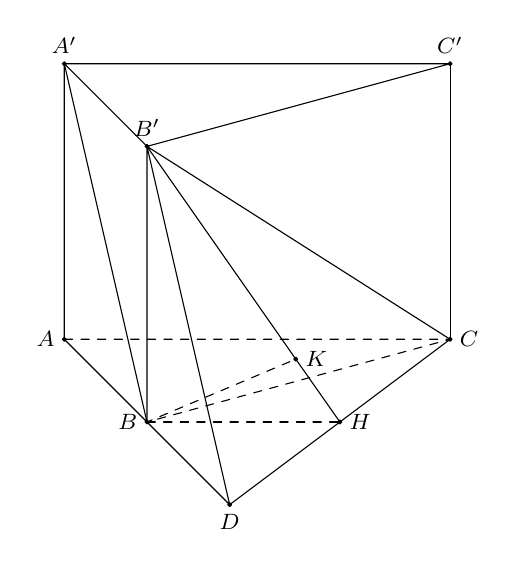
\begin{tikzpicture}[scale=0.7, font=\footnotesize, line join=round, line cap=round, >=stealth]
					%%%%%%%%%%%%%%%%%%%%%%%%%%%%%%%%%
					\coordinate (A) at (0,3);
					\coordinate (B) at (1.5,1.5);
					\coordinate (C) at (7,3);
					\coordinate (D) at (3,0);
					\coordinate (A') at (0,8);
					\coordinate (B') at (1.5,6.5);
					\coordinate (C') at (7,8);
					\coordinate (H) at (5,1.5);
					\coordinate (K) at (4.2,2.64);
					%%%%%%%%%%%%%%%%%%%%%%%%%%%%%%%%%
					\begin{scope}[dashed]
						\draw (A) -- (C)-- (B) -- (K);
						\draw (B) -- (H);
					\end{scope}
					\draw (A) -- (B) -- (A') --(A);
					\draw (A') -- (B') -- (B) --(D) -- (B') -- (C') -- (A');
					\draw (D) -- (H) -- (C) --(B') -- (K) -- (H); 
					\draw (C) --(C'); 
					%%%%%%%%%%%%%%%%%%%%%%%%%%%%%%%%%
					\filldraw [black] (0,3) circle (1pt) node[left] {$A$};
					\filldraw [black] (1.5,1.5) circle (1pt) node[left] {$B$};
					\filldraw [black] (7,3) circle (1pt) node[right] {$C$};
					\filldraw [black] (3,0) circle (1pt) node[below] {$D$};
					\filldraw [black] (0,8) circle (1pt) node[above] {$A'$};
					\filldraw [black] (1.5,6.5) circle (1pt) node[above] {$B'$};
					\filldraw [black] (7,8) circle (1pt) node[above] {$C'$};
					\filldraw [black] (5,1.5) circle (1pt) node[right] {$H$};
					\filldraw [black] (4.2,2.64) circle (1pt) node[right] {$K$};
					%%%%%%%%%%%%%%%%%%%%%%%%%%%%%%%%%
			\end{tikzpicture}}
			\noindent Từ (1) và (2) $\Rightarrow BK\perp \left( B'CD \right)\Rightarrow \mathrm{d} \left( A'B,B'C \right)=\mathrm{d} \left( B,\left( B'CD \right) \right)=BK$.\\
			$\Delta B'BH$ vuông tại $B$ có $BK$ là đường cao $\Rightarrow \dfrac{1}{BK^2}=\dfrac{1}{B'B^2}+\dfrac{1}{BH^2}=\dfrac{1}{a^2}+\dfrac{1}{\dfrac{a^2}{4}}=\dfrac{5}{a^2}$ \\ 
			$\Rightarrow BK=\dfrac{a\sqrt{5}}{5}$ hay $\mathrm{d} \left( A'B,B'C \right)=\dfrac{a\sqrt{5}}{5}$. 
		}
	\end{ex}
	
	\begin{ex}%[Đỗ Minh Phúc]%[1K7YQ-1]%
		Cho khối lập phương có cạnh bằng $\sqrt{2}$. Thể tích khối lập phương đã cho bằng
		\choice
		{\True $2\sqrt{2}$}
		{$3\sqrt{2}$}
		{$\dfrac{2\sqrt{2}}{3}$}
		{$4\sqrt{2}$}
		\loigiai{
			Thể tích khối lập phương đã cho bằng $V=\left(\sqrt{2}\right)^3=2\sqrt{2}$.}
	\end{ex}
	
	\begin{ex}%[Đỗ Minh Phúc]%[1K7BQ-3]%
		Cho hình chóp $S.ABC$ có đáy $ABC$ là tam giác vuông tại $A$, $AB=a$, $AC=a\sqrt{2}$. Biết thể tích khối chóp $S.ABC$ bằng $\dfrac{a^3}{2}$. Khoảng cách từ $S$ đến mặt phẳng $\left(ABC\right)$ bằng
		\choice
		{$\dfrac{a\sqrt{2}}{6}$}
		{$\dfrac{a\sqrt{2}}{2}$}
		{\True $\dfrac{3a\sqrt{2}}{2}$}
		{$\dfrac{3a\sqrt{2}}{4}$}
		\loigiai{Ta có $V_{S.ABC}=\dfrac{1}{3}\mathrm{d}\left(S,\left(ABC\right)\right)\cdot S_{ABC}\Leftrightarrow \mathrm{d}\left(S,\left(ABC\right)\right)=\dfrac{3V_{S.ABC}}{S_{ABC}}=\dfrac{3a^3}{2}:\dfrac{a^2\sqrt{2}}{2}=\dfrac{3a\sqrt{2}}{2}$.\\
			Vậy khoảng cách từ $S$ đến mặt phẳng $\left(ABC\right)$ bằng $\dfrac{3a\sqrt{2}}{2}$.}
	\end{ex}
	
	\begin{ex}%[Đỗ Minh Phúc]%[1K7BQ-3]%
		Cho khối lăng trụ tam giác đều có cạnh đáy bằng $3\mathrm{\,cm}$ và thể tích bằng $\dfrac{81}{4}\mathrm{\,cm}^3$. Khi đó độ dài cạnh bên của khối lăng trụ đã cho bằng 
		\choice
		{$3 \mathrm{\,cm} $}
		{\True $3\sqrt 3 \mathrm{\,cm}$}
		{$4\mathrm{\,cm}$}
		{$3\sqrt 2 \mathrm{\,cm}$}
		\loigiai{ 
			Ta có diện tích đáy $S=\dfrac{9\sqrt 3}{4}$.\\
			Vậy cạnh bên $h=\dfrac{V}{S}=\dfrac{\dfrac{81}{4}}{\dfrac{9\sqrt 3}{4}}=3\sqrt 3 $.}
	\end{ex}
	
	\begin{ex}%[Đỗ Minh Phúc]%[1K7BQ-1]%
		Cho hình chóp tứ giác $S.ABCD$ có đáy $ABCD$ là hình vuông cạnh $a$, cạnh bên $SA$ vuông góc với mặt đáy và $SA=a\sqrt{3}$. Tính thể tích $V$ của khối chóp $S.ABCD$.
		\choice
		{ $V=\dfrac{a^3\sqrt{3}}{6}$ }
		{ $V=a^3\sqrt{3}$ }
		{ $V=\dfrac{a^3\sqrt{3}}{4}$ }
		{\True $V=\dfrac{a^3\sqrt{3}}{3}$ }
		\loigiai
		{
			\immini{Ta có $V=\dfrac{1}{3}{S_{ABCD}}\cdot SA=\dfrac{1}{3}a^2\cdot a\sqrt{3}=\dfrac{a^3\sqrt{3}}{3}$.}
			{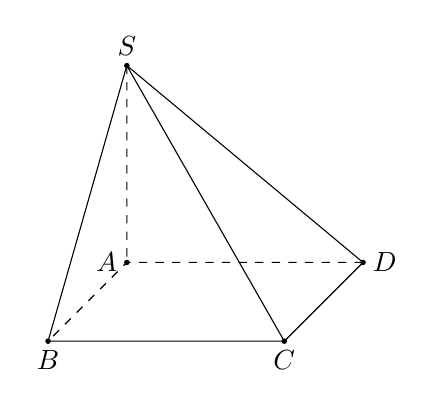
\begin{tikzpicture}[scale=1]
					\coordinate [label=above:$S$] (S) at (0,2.5);
					\coordinate [label=left:$A$] (A) at (0,0);
					\coordinate [label=below:$B$] (B) at (-1,-1);
					\coordinate [label=below:$C$] (C) at (2,-1);
					\coordinate [label=right:$D$] (D) at (3,0);
					\foreach \point in {A,B,C,D,S} \fill[black] (\point) circle (1pt);
					\draw[dashed] (D)--(A)--(B) (S)--(A);
					\draw (B)--(C)--(D)--(S)--(B) (S)--(C);
			\end{tikzpicture}}
		}
	\end{ex}
	
	\begin{ex}%[Đỗ Minh Phúc]%[1K7BQ-1]%
		Cho hình chóp $ S.ABCD$ có đáy là hình vuông cạnh bằng $ 2a$. Tam giác $ SAB$ đều và nằm trong mặt phẳng vuông góc với mặt phẳng $(ABCD)$. Thể tích của khối chóp $ S.ABCD$ là 
		\choice
		{$\dfrac{a^3\sqrt 3}{2}$}
		{\True $\dfrac{4a^3\sqrt 3}{3}$}
		{$\dfrac{a^3\sqrt 3}{4}$}
		{$ 4a^3\sqrt 3 $}
		\loigiai{
			\begin{center}
				\begin{tikzpicture}[declare function={a=2;b=4;h=4;},line join=round]
					\path (0,0) coordinate (B)
					(35:a) coordinate (A)
					(b,0) coordinate (C)
					($(C)-(B)+(A)$) coordinate (D)
					($(A)!1/2!(B)$) coordinate (H)
					($(H)+(90:h)$) coordinate (S);
					\draw (B)--(C)--(D)--(S)--cycle  (S)--(C);
					\draw[dashed] (A)--(D) (H)--(S)--(A)--(B);
					\foreach \t/\g in {A/150,B/-90,C/-90,D/0,S/90,H/180}{
						\draw[fill=white] (\t) circle (1pt) node[shift={(\g:7pt)},font=\scriptsize]{$ \t $};
					}
				\end{tikzpicture}
			\end{center}
			Gọi $H$ là trung điểm của cạnh $ AB$. \\
			Vì tam giác $SAB$ đều, cạnh bằng $2a$ nên $SH\perp AB$ và $ SH=a\sqrt{3}$.\\
			Ta có $\heva{& (SAB)\perp (ABCD)\\ & (SAB) \cap (ABCD)\\ & SH \perp AB,\, SH \subset (SAB)}
			\Rightarrow SH\perp(ABCD)$.\\
			Vậy $V_{S.ABCD}=\dfrac{1}{3}SH\cdot S_{ABCD}=\dfrac{1}{3}\cdot a\sqrt{3}\cdot (2a)^2=\dfrac{4a^3\sqrt 3}{3}$.}
	\end{ex}
	
	\begin{ex}%[Đỗ Minh Phúc]%[1K7BQ-1]%
		Cho khối lăng trụ tam giác $ ABC.A'B'C'$ có thể tích $ V=3$. Thể tích khối chóp $ A'.AB'C'$ là
		\choice
		{$\dfrac{1}{2}$}
		{\True $ 1$}
		{$ 3$}
		{$\dfrac{1}{3}$}
		\loigiai{ 
			\immini{
				Ta có \[V_{A'.AB'C'}=V_{A.A'B'C'}=\dfrac{1}{3}S_{A'B'C'}\cdot\mathrm{d}\left(A,\,\left(A'B'C'\right)\right)=\dfrac{1}{3}V=1.\]
			}{
				\begin{tikzpicture}[scale=0.7, font=\footnotesize, line join=round, line cap=round, >=stealth]
					\path
					(0,0) coordinate (A')
					(2,-2) coordinate (B')
					(5,0) coordinate (C') 
					(1,-.5)coordinate (H) ;
					\path (H)+(0,5) coordinate(A);
					\coordinate (B) at ($(A)+(B')-(A')$);
					\coordinate (C) at ($(A)+(C')-(A')$);
					\draw[dashed] (A')--(C') (A)--(H);
					\draw(A)--(B)--(C) (A)--(A')--(B')--(C')--(C) (B')--(B) (A)--(C);
					\foreach \p/\g in {A'/180,B'/-90,C'/0,A/180,B/-45,C/0}\draw[fill=black] (\p) circle (1pt)node[shift={(\g:.4)}]{$\p$};
			\end{tikzpicture}}
			
		}
	\end{ex}
	
	\begin{ex}%[Đỗ Minh Phúc]%[1K7BQ-1]%%
		Cho hình chóp $S.ABC$ có đáy là tam giác đều cạnh $a$. Cạnh bên $SC$ vuông góc với mặt phẳng $(ABC)$, $SC=a$. Thể tích khối chóp $S.ABC$ bằng
		\choice
		{$\dfrac{a^3\sqrt{3}}{3}$}
		{\True $\dfrac{a^3\sqrt{3}}{12}$}
		{$\dfrac{a^3\sqrt{3}}{9}$}
		{$\dfrac{a^3\sqrt{2}}{12}$}
		\loigiai{
			Ta có $V_{S.ABC}=\dfrac{1}{3}\cdot S_{\triangle ABC}\cdot SC=\dfrac{1}{3}\cdot \dfrac{a^2\sqrt{3}}{4}\cdot a=\dfrac{a^3\sqrt{3}}{12}$.}
	\end{ex}
	
	\begin{ex}%[Đỗ Minh Phúc]%[1K7KQ-1]%
		Cho hình lăng trụ đứng $ABC.A'B'C'$ có đáy là tam giác đều cạnh $2a$. Mặt phẳng $\left(AB'C'\right)$ tạo với mặt đáy góc $30^\circ$. Tính theo $a$ thể tích của khối lăng trụ $ABC.A'B'C'$.
		\choice
		{ $V=\dfrac{3a^3\sqrt{3}}{8}$ }
		{\True $V=a^3\sqrt{3}$ }
		{ $V=\dfrac{3a^3\sqrt{3}}{4}$ }
		{ $V=\dfrac{a^3\sqrt{3}}{8}$ }
		\loigiai{
			\immini{Gọi $I$ là trung điểm của $B'C'$\\
				Ta có $\left\{ \begin{aligned}
					& \left(A'B'C'\right)\cap \left(AB'C'\right)=B'C' \\ 
					& A'I\subset\left(A'B'C'\right), A'I\perp B'C' \\ 
					& AI\subset\left(AB'C'\right), AI\perp B'C' \\ 
				\end{aligned} \right.$\\
				$\Rightarrow \left(\left(AB'C'\right);\left(A'B'C'\right)\right)=\widehat{AIA'}=30^\circ$.\\
				Diện tích ${\Delta ABC}$ là  $S_{\Delta ABC}=\left(2a\right)^2\cdot\dfrac{\sqrt{3}}{4}=a^2\sqrt{3}$.\\
				Ta có $A'I=2a\cdot\dfrac{\sqrt{3}}{2}=a\sqrt{3}\Rightarrow AA'=A'I\cdot\tan 30^\circ=a\sqrt{3}\cdot\dfrac{1}{\sqrt{3}}=a$.\\
				Vậy $V=S_{\Delta ABC}\cdot AA'=a^2\sqrt{3}\cdot a=a^3\sqrt{3}$.}
			{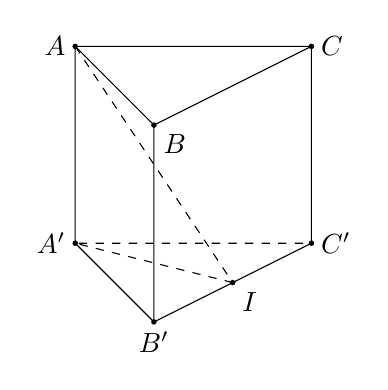
\begin{tikzpicture}[scale=1]
					\coordinate [label=left:$A$] (A') at (0,2.5);
					\coordinate [label=left:$A'$] (A) at (0,0);
					\coordinate [label=below right:$B$] (B') at (1,1.5);
					\coordinate [label=below:$B'$] (B) at (1,-1);
					\coordinate [label=right:$C$] (C') at (3,2.5);
					\coordinate [label=right:$C'$] (C) at (3,0);
					\coordinate [label=below right:$I$] (I) at (2,-0.5);
					\foreach \point in {A,B,C,A',B',C',I} \fill[black] (\point) circle (1pt);
					\draw[dashed] (I)--(A)--(C) (A')--(I);
					\draw (A)--(B)--(C)--(C')--(A')--(B')--(C') (A)--(A') (B)--(B');
			\end{tikzpicture}}
		}
	\end{ex}
	
	\begin{ex}%[Đỗ Minh Phúc]%[1K7KQ-1]%	
		Cho hình chóp $S.ABCD$ có đáy $ABCD$ là hình bình hành. Mặt bên $SAB$ là tam giác đều cạnh $a\sqrt{3}$, tam giác $ABC$ vuông tại $A$ có $AC=a$, góc giữa đường thẳng $AD$ và mặt phẳng $\left( SAB \right)$ bằng $60^\circ$. Thể tích của khối chóp $S.ABCD$ là
		\choice
		{ $a^3$}
		{ $\dfrac{a^3\sqrt{3}}{2}$}
		{ $\dfrac{3a^3}{4}$}
		{\True $\dfrac{3a^3}{2}$}
		\loigiai{
			\immini{
				Trong $\triangle ABC$ vuông tại $A$ có\\ $BC=\sqrt{A{C^2}+A{B^2}}=\sqrt{{{\left( a\sqrt{3} \right)}^2}+a^2}=2a$.\\
				Góc giữa đường thẳng $AD$ và mặt phẳng $\left( SAB \right)$ bằng $60^\circ $, ta có\\
				$\sin 60{}^\circ =\dfrac{\mathrm{d}\left( D,\left( SAB \right) \right)}{AD}\Leftrightarrow \mathrm{d}\left( D,\left( SAB \right) \right)=\sin 60^\circ \cdot AD=a\sqrt{3}$.
				Diện tích của tam giác đều $SAB$ là $${S_{\Delta SAB}}=\dfrac{1}{2}\cdot SA\cdot SB\cdot \sin 60{}^\circ =\dfrac{1}{2}\cdot \sqrt{3}a\cdot \sqrt{3}a\cdot \dfrac{\sqrt{3}}{2}=\dfrac{3a^2\sqrt{3}}{4}.$$
			}{
				\begin{tikzpicture}[scale=0.6, font=\footnotesize, line join=round, line cap=round, >=stealth]
					\path 
					(-2.3,0.61) coordinate (A)
					(-4.62,-1.71) coordinate (B)	
					(1.92,-1.71) coordinate (C)	
					(4.23,0.61) coordinate (D)	
					(-1.8,6.01) coordinate (S)	
					(-0.19,-0.55) coordinate (O)
					;
					\draw (S)--(B) (S)--(C) (S)--(D) (B)--(C) (C)--(D) ;
					\draw[dashed] (S)--(A) (A)--(B) (D)--(A);
					\foreach \x/\g in{A/150,B/-100,C/-80,D/-80,S/90}
					\fill[black](\x) circle (2pt)
					($(\x)+(\g:5mm)$) node{\small $\x$};
				\end{tikzpicture} 
			}
			\noindent
			Thể tích của khối chóp $S.ABC$ là $${V_{D.SAB}}=\dfrac{1}{3}\cdot \mathrm{d}\left( D; \left( SAB \right) \right)\cdot {S_{\triangle SAB}}=\dfrac{1}{3}\cdot \dfrac{3a^2\sqrt{3}}{4}\cdot a\sqrt{3}=\dfrac{3a^3}{4}.$$
			Vậy thể tích của khối chóp $S.ABCD$ là $${V_{S.ABCD}}=2{V_{S.ABD}}=2\cdot \dfrac{3a^3}{4}=\dfrac{3a^3}{2}.$$
		}
	\end{ex}
\Closesolutionfile{ans}
\begin{indapan}{10}
	{ans/ans-1K7-27-OTC}
\end{indapan}
	
	
